% 第6章 高阶归纳类型 / Chapter 6: Higher Inductive Types
% 翻译状态:已完成
% 译者:MT
% 审校:

\label{cha:hits}

\index{type!higher inductive|(}%
\indexsee{inductive!type!higher}{type, higher inductive}%
\indexsee{higher inductive type}{type, higher inductive}%

\section{引言}
\label{sec:intro-hits}

\index{generation!of a type, inductive|(}

与我们在\cref{cha:induction}中讨论的一般归纳类型一样,\emph{高阶归纳类型}是由某些构造子生成新类型的一般模式。
但与普通归纳类型不同的是,在定义高阶归纳类型时,我们可以有不仅生成该类型的\emph{点},而且还生成该类型中的\emph{道路}和高阶道路的``构造子''。
\index{type!circle}%
\indexsee{circle type}{type,circle}%
例如,我们可以考虑由以下构造子生成的高阶归纳类型 $\Sn^1$:
\begin{itemize}
\item 一个点 $\base:\Sn^1$,以及
\item 一条道路 $\lloop : {\id[\Sn^1]\base\base}$。
\end{itemize}
这应该被视为完全类似于将 $\bool$ 定义为由以下构造子生成:
\begin{itemize}
\item 一个点 $\bfalse:\bool$,以及
\item 一个点 $\btrue:\bool$,
\end{itemize}
或者将 $\nat$ 定义为由以下构造子生成:
\begin{itemize}
\item 一个点 $0:\nat$,以及
\item 一个函数 $\suc:\nat\to\nat$。
\end{itemize}
当我们将类型视为高阶群胚时,这种更一般的``生成''概念是非常自然的:
由于高阶群胚是具有道路和高阶道路以及点的``多类型对象'',我们应该允许各个维度的``生成元''。

我们将普通类型的构造子(如 $\base$)称为\define{点构造子}
\indexdef{constructor!point}%
\indexdef{point!constructor}%
或\emph{普通构造子},而将其他构造子(如 $\lloop$)称为\define{道路构造子}
\indexdef{constructor!path}%
\indexdef{path!constructor}%
或\emph{高阶构造子}。
每个道路构造子必须指定道路的起点和终点,我们分别称之为其\define{源}
\indexdef{source!of a path constructor}%
和\define{靶};
\indexdef{target!of a path constructor}%
对于 $\lloop$,源和靶都是 $\base$。

注意,像 $\lloop$ 这样的道路构造子生成一个恒等类型的\emph{新}居民,它(至少\emph{先验}地)不等于任何先前存在的这类居民。
特别是,$\lloop$ \emph{先验}地不等于 $\refl{\base}$(尽管证明它们确实不相等需要一些思考;见\cref{thm:loop-nontrivial})。
这就是将 $\Sn^1$ 与普通归纳类型 \unit 区分开来的地方。

关于这种推广,有一些重要的要点需要说明。

\index{free!generation of an inductive type}%
首先,``生成''这个词应该认真对待,就像一个群可以由某个集合自由生成一样。
特别是,由于高阶群胚具有道路和高阶道路上的\emph{运算},当这样一个对象被某些构造子``生成''时,这些运算会创建更多不直接来自构造子本身的道路。
例如,在高阶归纳类型 $\Sn^1$ 中,构造子 $\lloop$ 不是从 $\base$ 到 $\base$ 的唯一非平凡道路;我们还有``$\lloop\ct\lloop$''、``$\lloop\ct\lloop\ct\lloop$''等等,以及 $\opp{\lloop}$,等等,它们都是不同的。
这可能看起来太明显以至于不值得一提,但这与``普通''归纳类型的行为不同,在普通归纳类型中,人们可以期望在归纳类型中只看到由构造子直接``放入''的东西。

其次,这种生成确实是\emph{自由}生成:高阶归纳类型在技术上不允许我们施加``公理'',例如强制``$\lloop\ct\lloop$''等于 $\refl{\base}$。
然而,在 $\infty$-群胚的世界中,%
\index{.infinity-groupoid@$\infty$-groupoid}
``自由生成''和``表示''之间几乎没有区别,
\index{presentation!of an infinity-groupoid@of an $\infty$-groupoid}%
\index{generation!of an infinity-groupoid@of an $\infty$-groupoid}%
因为我们可以通过添加一个将它们关联起来的新 2 维生成元(例如,$\base=\base$ 中的道路 $\lloop\ct\lloop = \refl{\base}$)使两条道路\emph{同伦}相等。
当然,我们确实需要担心这个新生成元是否应该满足它自己的``公理'',等等,但原则上任何``表示''都可以通过将公理变成构造子来转化为``自由''的。
正如我们将看到的,通过添加``截断构造子'',我们也可以使用高阶归纳类型来表达经典概念,如群表示。

第三,即使高阶归纳类型包含生成该类型\emph{中}道路的``构造子'',它仍然是\emph{单个}类型的归纳定义。
特别是,正如我们将看到的,被赋予泛性质(像往常一样通过归纳原理表达)的是高阶归纳类型本身,而\emph{不是}其恒等类型。
高阶归纳类型的恒等类型保留任何恒等类型的通常归纳原理(即道路归纳),并不获得任何新的归纳原理。

因此,以具体方式识别高阶归纳类型的恒等类型可能是非平凡的,这与\cref{cha:basics}中我们能够给出恒等类型在所有传统类型形成运算下行为的显式描述形成对比。
例如,在 $\Sn^1$ 中是否有任何从 $\base$ 到 $\base$ 的道路不是简单地由 $\lloop$ 及其逆的复合组成的?
直觉上,答案似乎应该是否定的(确实是),但证明这一点并非平凡。
事实上,这类问题很快就把我们带到诸如计算球面的同伦群这样的问题,这是代数拓扑中一个长期存在的问题,目前还没有已知的简单公式。
同伦类型论为这类问题带来了新的强大视角,但它也要求类型论变得像这些问题的答案一样复杂。

\index{dimension!of path constructors}%
第四,构造子的``维度''(即它们是输出点、道路、道路之间的道路等)与结果类型在哪些维度具有非平凡同伦没有直接关系。
作为一个简单的例子,如果一个归纳类型 $B$ 有一个类型为 $A\to B$ 的构造子,那么 $A$ 中的任何道路和高阶道路都会导致 $B$ 中的道路和高阶道路,即使该构造子根本不是``高阶''构造子。
高阶构造子也会发生同样的事情:具有类型为 $A\to (\id[B]xy)$ 的构造子不仅意味着 $A$ 的点产生 $B$ 中从 $x$ 到 $y$ 的道路,而且 $A$ 中的道路产生这些道路之间的道路,等等。
正如我们将看到的,这种可能性是高阶归纳类型大部分威力的来源。

另一方面,甚至没有在其输入中包含高阶类型的构造子也可能生成``意外的''高阶道路。
例如,在由以下构造子生成的 2 维球面 $\Sn^2$ 中
\symlabel{s2a}
\index{type!2-sphere}%
\begin{itemize}
\item 一个点 $\base:\Sn^2$,以及
\item 一条 2 维道路 $\surf:\refl{\base} = \refl{\base}$ 在 ${\base=\base}$ 中,
\end{itemize}
存在一条从 $\refl{\refl{\base}}$ 到自身的非平凡\emph{3 维道路}。
拓扑学家会认出这条道路是\emph{Hopf 纤维化}的一种体现。
从范畴论的角度看,这与上面提到的 $\Sn^1$ 不仅包含 $\lloop$ 还包含 $\lloop\ct\lloop$ 等等是同一种现象:只是在\emph{高阶}群胚中,存在提升维度的\emph{运算}。
事实上,我们在\cref{sec:equality}中已经看到了许多这样的运算:结合律和单位律不仅仅是性质,而是运算,其输入是 1-道路,输出是 2-道路。

\index{generation!of a type, inductive|)}%

% In US Trade format it wants a page break here but then it stretches the above itemize,
% so we give it some stretchable space to use if it wants to.
\vspace*{0pt plus 20ex}

\section{归纳原理与依赖道路}
\label{sec:dependent-paths}

当我们将像圆周这样的高阶归纳类型描述为由某些构造子生成时,我们必须通过给出类似于\cref{cha:typetheory}中基本类型构造子的规则来解释这意味着什么。
构造子本身给出\emph{引入}规则,但解释\emph{消去}规则,即归纳和递归原理,需要更多思考。
在本书中,我们不试图给出什么构成``高阶归纳定义''以及如何从这样的定义中提取消去规则的一般表述——事实上,这是一个微妙的问题,也是当前研究的主题。
相反,我们将依靠一些一般性的非形式讨论和大量例子。

\index{type!circle}%
\index{recursion principle!for S1@for $\Sn^1$}%
递归原理通常很容易描述:给定任何具有与构造子赋予所讨论的高阶归纳类型相同结构的类型,存在一个将构造子映射到该结构的函数。
例如,对于 $\Sn^1$,递归原理说如果给定任何类型 $B$,配备一个点 $b:B$ 和一条道路 $\ell:b=b$,则存在一个函数 $f:\Sn^1\to B$ 使得 $f(\base)=b$ 且 $\apfunc f (\lloop) = \ell$。

\index{computation rule!for S1@for $\Sn^1$}%
\index{equality!definitional}%
后两个等式是\emph{计算规则}。
\index{computation rule!for higher inductive types|(}%
\index{computation rule!propositional|(}%
然而,有一个问题是这些计算规则是判断等式还是命题等式(道路)。
对于普通归纳类型,我们毫不犹豫地使它们成为判断的,尽管我们在\cref{cha:induction}中看到使它们成为命题的仍然会产生等价的类型。
在普通情况下,人们可以论证计算规则确实是\emph{定义}等式,就像引言中描述的直觉意义一样。

\index{equality!judgmental}%
对于高阶归纳类型,这就不那么清楚了。
此外,由于运算 $\apfunc f$ 并不真正是类型论的基本部分,而是我们使用恒等类型的归纳原理\emph{定义}的东西(我们可能以某种其他等价的方式定义),在\emph{判断}等式中显式引用它似乎不合适。
判断等式是演绎系统的一部分,它不应该依赖于我们可能在该系统\emph{内部}做出的特定定义选择。
还有语义和实现问题需要考虑;参见注释。

将高阶归纳类型的\emph{点}构造子的计算规则设为判断的似乎是没有问题的。
在上面的例子中,这意味着我们判断地有 $f(\base)\jdeq b$。
这种选择有利于高阶归纳类型的计算观点。
此外,它也大大简化了我们的生活,因为否则第二个计算规则 $\apfunc f (\lloop) = \ell$ 作为命题等式甚至不会是良型的;我们需要将一边或另一边与 $f(\base)$ 和 $b$ 的指定恒等式组合。
(当然,当我们开始讨论更高维度的道路时,这类问题最终会出现,但这在这里不会引起我们太大的关注。另见\cref{sec:hubs-spokes}。)
因此,我们将点构造子的计算规则设为判断的,而道路和高阶道路的计算规则设为命题的。%
\footnote{特别是,用\cref{sec:types-vs-sets}的语言来说,这意味着我们的高阶归纳类型是\emph{规则}(指定我们如何引入这类类型及其元素、它们的归纳原理以及它们对点构造子的计算规则)和\emph{公理}(道路构造子的计算规则,断言某些恒等类型由其他未指定的项居住)的混合。
我们可以希望最终会有一个更好的类型论,其中高阶归纳类型像泛等性一样,将只使用规则而不使用公理来呈现。%
\indexfoot{axiom!versus rules}%
\indexfoot{rule!versus axioms}%
}

\begin{rmk}\label{rmk:defid}
回想一下,对于普通归纳类型,我们将递归定义函数的计算规则不仅视为判断等式,而且视为\emph{定义}等式,因此我们可以使用记号 $\defeq$。
例如,截断前驱\index{predecessor!function, truncated}函数 $p:\nat\to\nat$ 由 $p(0)\defeq 0$ 和 $p(\suc(n))\defeq n$ 定义。
对于高阶归纳类型,这种记号对于点构造子是合理的(例如 $f(\base)\defeq b$),但对于道路构造子可能会产生误导,因为像 $\ap f \lloop = \ell$ 这样的等式不是判断的。
因此,我们混合使用这些记号,改写为 $\ap f \lloop \defid \ell$,表示这种``定义的命题等式''。
\end{rmk}
\index{computation rule!for higher inductive types|)}%
\index{computation rule!propositional|)}%

\index{type!circle|(}%
\index{induction principle!for S1@for $\Sn^1$}%
现在,归纳原理(依赖消去子)呢?
回想一下,对于普通归纳类型 $W$,要通过归纳证明 $\prd{x:W} P(x)$,我们必须为 $W$ 的每个构造子指定一个作用于该构造子上方``纤维''的 $P$ 上的运算。
例如,如果 $W$ 是自然数 \nat,那么要通过归纳证明 $\prd{x:\nat} P(x)$,我们必须指定
\begin{itemize}
\item 构造子 $0:\nat$ 上方纤维中的一个元素 $b:P(0)$,以及
\item 对于每个 $n:\nat$,一个函数 $P(n) \to P(\suc(n))$。
\end{itemize}
第二个可以被视为\emph{位于}构造子 $\suc:\nat\to\nat$ \emph{上方}的函数``$P\to P$'',推广了 $b:P(0)$ 如何位于构造子 $0:\nat$ 上方。

因此,类似地,要证明 $\prd{x:\Sn^1} P(x)$,我们应该指定
\begin{itemize}
\item 构造子 $\base:\Sn^1$ 上方纤维中的一个元素 $b:P(\base)$,以及
\item 一条从 $b$ 到 $b$ 的道路``位于构造子 $\lloop:\base=\base$ 上方''。
\end{itemize}
注意,即使 $\Sn^1$ 包含除 $\lloop$ 之外的道路(如 $\refl{\base}$ 和 $\lloop\ct\lloop$),我们只需要指定一条位于构造子\emph{本身}上方的道路。
这表达了 $\Sn^1$ 是由其构造子``自由生成''的直觉。

然而,问题是道路``位于''另一条道路``上方''意味着什么。
它确实\emph{不}意味着简单地是一条道路 $b=b$,因为那将是纤维 $P(\base)$ 中的一条道路(拓扑上,一条位于 $\base$ 处的\emph{常值}道路上方的道路)。
实际上,我们在\cref{cha:basics}中已经回答了这个问题:在\cref{lem:mapdep}之前的讨论中,我们得出结论,从 $u:P(x)$ 到 $v:P(y)$ 的位于 $p:x=y$ 上方的道路可以由纤维 $P(y)$ 中的道路 $\trans p u = v$ 表示。
由于我们将在本章大量使用这种\define{依赖道路}
\index{path!dependent}%
,我们为它们引入一个特殊记号:
\begin{equation}
  (\dpath P p u v) \defeq (\transfib{P} p u = v).\label{eq:dpath}
\end{equation}

\begin{rmk}
还有其他可能的方式来定义依赖道路。
例如,我们可以考虑 $u = \trans{(\opp p)}{v}$ 而不是 $\trans p u = v$。
我们也可以将其作为更一般的``异质等式''的特例获得,
\index{heterogeneous equality}%
\index{equality!heterogeneous}%
或者直接定义为归纳类型族。
所有这些定义都导致等价的类型,所以从这个意义上说我们选择哪个并不重要。
然而,选择 $\trans p u = v$ 作为定义使得推导关于依赖道路的其他结论最容易,例如 $\apdfunc{f}$ 产生它们的事实,或者我们可以使用\cref{sec:computational}中的传输引理在特定类型族中计算它们。
\end{rmk}

有了依赖道路的概念,我们现在可以更精确地陈述 $\Sn^1$ 的归纳原理:给定 $P:\Sn^1\to\type$ 以及
\begin{itemize}
\item 一个元素 $b:P(\base)$,以及
\item 一条道路 $\ell : \dpath P \lloop b b$,
\end{itemize}
存在一个函数 $f:\prd{x:\Sn^1} P(x)$ 使得 $f(\base)\jdeq b$ 且 $\apd f \lloop = \ell$。
像非依赖情况一样,我们说 $f$ 由 $f(\base)\defeq b$ 和 $\apd f \lloop \defid \ell$ 定义。

\begin{rmk}\label{rmk:varies-along}
  当非形式地描述这个归纳原理的应用时,我们将其视为将目标``对所有 $x:\Sn^1$ 有 $P(x)$''分成两种情况,我们有时会用诸如``当 $x$ 是 $\base$ 时''和``当 $x$ 沿 $\lloop$ 变化时''这样的短语分别引入。
  \index{vary along a path constructor}%
  ``沿道路变化''没有被赋予具体的数学含义:它只是表示证明相应部分开始的便捷方式;参见\cref{thm:S1-autohtpy}的一个例子。
\end{rmk}

拓扑上,$\Sn^1$ 的归纳原理可以如\cref{fig:topS1ind}所示进行可视化。
给定圆周上的一个纤维化(在图中是一个环面),定义这个纤维化的一个截面等同于给出 $\base$ 上方纤维中的一个点 $b$ 以及一条从 $b$ 到 $b$ 的位于 $\lloop$ 上方的道路。
我们使用依赖道路定义从类型论角度解释这一点的方式如\cref{fig:ttS1ind}所示:从 $b$ 到 $b$ 的位于 $\lloop$ 上方的道路由 $\base$ 上方纤维中从 $\trans \lloop b$ 到 $b$ 的道路表示。

\begin{figure}
  \centering
  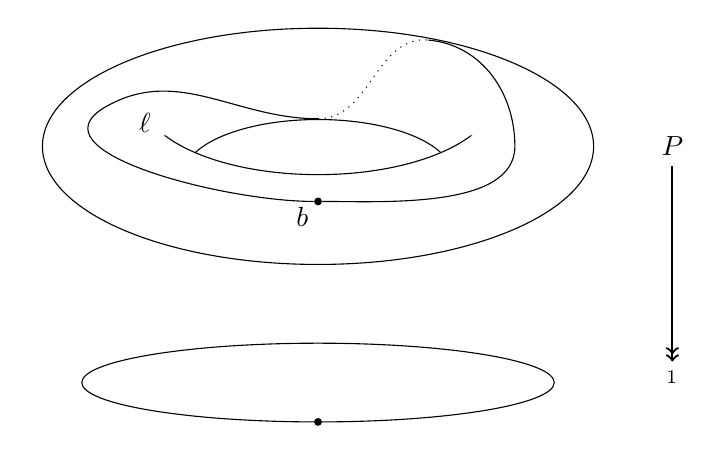
\begin{tikzpicture}
    \draw (0,0) ellipse (3 and .5);
    \draw (0,3) ellipse (3.5 and 1.5);
    \begin{scope}[yshift=4]
      \clip (-3,3) -- (-1.8,3) -- (-1.8,3.7) -- (1.8,3.7) -- (1.8,3) -- (3,3) -- (3,0) -- (-3,0) -- cycle;
      \draw[clip] (0,3.5) ellipse (2.25 and 1);
      \draw (0,2.5) ellipse (1.7 and .7);
    \end{scope}
    \node (P) at (4.5,3) {$P$};
    \node (S1) at (4.5,0) {$\Sn^1$};
    \draw[->>,thick] (P) -- (S1);
    \node[fill,circle,inner sep=1pt,label={below right:$\base$}] at (0,-.5) {};
    \node at (-2.6,.6) {$\lloop$};
    \node[fill,circle,\OPTblue,inner sep=1pt] (b) at (0,2.3) {};
    \node[\OPTblue] at (-.2,2.1) {$b$};
      \begin{scope}
        \draw[\OPTblue] (b) to[out=180,in=-150] (-2.7,3.5) to[out=30,in=180] (0,3.35);
        \draw[\OPTblue,dotted] (0,3.35) to[out=0,in=175] (1.4,4.35);
        \draw[\OPTblue] (1.4,4.35) to[out=-5,in=90] (2.5,3) to[out=-90,in=0,looseness=.8] (b);
      \end{scope}
      \node[\OPTblue] at (-2.2, 3.3) {$\ell$};
  \end{tikzpicture}
  \caption{$\Sn^1$ 的拓扑归纳原理}
  \label{fig:topS1ind}
\end{figure}

\begin{figure}
  \centering
  \begin{tikzpicture}
    \draw (0,0) ellipse (3 and .5);
    \draw (0,3) ellipse (3.5 and 1.5);
    \begin{scope}[yshift=4]
      \clip (-3,3) -- (-1.8,3) -- (-1.8,3.7) -- (1.8,3.7) -- (1.8,3) -- (3,3) -- (3,0) -- (-3,0) -- cycle;
      \draw[clip] (0,3.5) ellipse (2.25 and 1);
      \draw (0,2.5) ellipse (1.7 and .7);
    \end{scope}
    \node (P) at (4.5,3) {$P$};
    \node (S1) at (4.5,0) {$\Sn^1$};
    \draw[->>,thick] (P) -- (S1);
    \node[fill,circle,inner sep=1pt,label={below right:$\base$}] at (0,-.5) {};
    \node at (-2.6,.6) {$\lloop$};
    \node[fill,circle,\OPTblue,inner sep=1pt] (b) at (0,2.3) {};
      \node[\OPTblue] at (-.3,2.3) {$b$};
      \node[fill,circle,\OPTpurple,inner sep=1pt] (tb) at (0,1.8) {};
      % \draw[\OPTpurple,dashed] (b) to[out=0,in=0,looseness=5] (0,4) to[out=180,in=180] (tb);
      \draw[\OPTpurple,dashed] (b) arc (-90:90:2.9 and 0.85) arc (90:270:2.8 and 1.1);
      \begin{scope}
        \clip (b) -- ++(.1,0) -- (.1,1.8) -- ++(-.2,0) -- ++(0,-1) -- ++(3,2) -- ++(-3,0) -- (-.1,2.3) -- cycle;
        \draw[\OPTred,dotted,thick] (.2,2.07) ellipse (.2 and .57);
        \begin{scope}
          % \draw[clip] (b) -- ++(.1,0) |- (tb) -- ++(-.2,0) -- ++(0,-1) -| ++(3,3) -| (b);
          \clip (.2,0) rectangle (-2,3);
          \draw[\OPTred,thick] (.2,2.07) ellipse (.2 and .57);
        \end{scope}
      \end{scope}
      \node[\OPTred] at (1,1.2) {$\ell: \trans \lloop b=b$};
  \end{tikzpicture}
  \caption{$\Sn^1$ 的类型论归纳原理}
  \label{fig:ttS1ind}
\end{figure}

当然,我们期望能够从归纳原理证明递归原理,通过取 $P$ 为常值类型族。
这确实是如此,尽管从依赖计算规则(涉及 $\apdfunc f$)导出 $\lloop$ 的非依赖计算规则(涉及 $\apfunc f$)出乎意料地有些棘手。

\begin{lem}\label{thm:S1rec}
  \index{recursion principle!for S1@for $\Sn^1$}%
  \index{computation rule!for S1@for $\Sn^1$}%
  如果 $A$ 是一个类型,配备 $a:A$ 和 $p:\id[A]aa$,则存在一个函数 $f:\Sn^1\to{}A$ 满足
  \begin{align*}
    f(\base)&\defeq a \\
    \apfunc f(\lloop)&\defid p.
  \end{align*}
\end{lem}
\begin{proof}
  我们想将 $\Sn^1$ 的归纳原理应用于常值类型族 $(\lam{x} A): \Sn^1\to \UU$。
  为此所需的假设是 $(\lam{x} A)(\base) \jdeq A$ 的一个点,我们有(即 $a:A$),以及 $\dpath {x \mapsto A}{\lloop} a a$ 中的一条依赖道路,或等价地 $\transfib{x \mapsto A}{\lloop} a = a$。
  后一个类型与 $p$ 所在的类型 $\id[A]aa$ 不同,但它与之等价,因为由\cref{thm:trans-trivial}我们有 $\transconst{A}{\lloop}{a} : \transfib{x \mapsto A}{\lloop} a= a$。
  因此,给定 $a:A$ 和 $p:a=a$,我们可以考虑复合
  \[\transconst{A}{\lloop}{a} \ct p:(\dpath {x \mapsto A}\lloop aa).\]
  应用归纳原理,我们得到 $f:\Sn^1\to A$ 使得
  \begin{align}
    f(\base) &\jdeq a \qquad\text{以及}\label{eq:S1recindbase}\\
    \apdfunc f(\lloop) &= \transconst{A}{\lloop}{a} \ct p.\label{eq:S1recindloop}
  \end{align}
  还需要导出等式 $\apfunc f(\lloop)=p$。
  然而,由\cref{thm:apd-const},我们有
  \[\apdfunc f(\lloop) = \transconst{A}{\lloop}{f(\base)} \ct \apfunc f(\lloop).\]
  将此与\eqref{eq:S1recindloop}结合并消去 $\transconstf$ 的出现(由\eqref{eq:S1recindbase}它们是相同的),我们得到 $\apfunc f(\lloop)=p$。
\end{proof}

% Similarly, in this case we speak of defining $f$ by $f(\base)\defeq a$ and $\ap f \lloop \defid p$.
我们还有一个相应的唯一性原理。

\begin{lem}\label{thm:uniqueness-for-functions-on-S1}
  \index{uniqueness!principle, propositional!for functions on the circle}%
  如果 $A$ 是一个类型且 $f,g:\Sn^1\to{}A$ 是两个映射,配备两个等式 $p,q$:
  \begin{align*}
    p:f(\base)&=_Ag(\base),\\
    q:\map{f}\lloop&=^{\lam{x} x=_Ax}_p\map{g}\lloop.
  \end{align*}
  则对所有 $x:\Sn^1$ 我们有 $f(x)=g(x)$。
\end{lem}
\begin{proof}
  我们将 $\Sn^1$ 的归纳原理应用于类型族 $P(x)\defeq(f(x)=g(x))$。
  当 $x$ 是 $\base$ 时,$p$ 正是我们所需的。
  当 $x$ 沿 $\lloop$ 变化时,我们需要
  \(p=^{\lam{x} f(x)=g(x)}_{\lloop} p,\)
  这由\cref{thm:transport-path,thm:dpath-path}可归约为 $q$。
\end{proof}

\index{universal!property!of S1@of $\Sn^1$}%
这两个引理蕴含圆周的期望泛性质:

\begin{lem}\label{thm:S1ump}
  对任意类型 $A$,我们有一个自然等价
  \[ (\Sn^1 \to A) \;\eqvsym\;
  \sm{x:A} (x=x).
  \]
\end{lem}
\begin{proof}
  我们有一个由 $f(g) \defeq (g(\base),\ap g \lloop)$ 定义的典范函数 $f:(\Sn^1 \to A) \to \sm{x:A} (x=x)$。
  反方向,我们有 $g:\sm{x:A} (x=x) \to (\Sn^1 \to A)$,它将一对 $(b,\ell)$ 映射到由圆周的递归原理给出的函数 $\Sn^1 \to A$。

  现在,由递归原理的计算规则,$f \circ g \htpy \idfunc$。
  而 $g \circ f \htpy \idfunc$ 由唯一性原理得出,
  因为 \((g \circ f)(\lloop) =^{\lam{x} x=_Ax}_{\refl{\base}} \lloop\),再次由圆周的递归原理的计算规则。
  因此,$f$ 有一个拟逆,从而是一个等价。
\end{proof}

\index{type!circle|)}%

如\cref{sec:htpy-inductive}中那样,我们可以证明\cref{thm:S1ump}的结论等价于具有带命题计算规则的归纳原理。
其他高阶归纳类型也满足类似于\cref{thm:S1rec,thm:S1ump}的引理;我们通常将其证明留给读者。
我们现在继续考虑许多例子。


\section{区间}
\label{sec:interval}

\index{type!interval|(defstyle}%
\indexsee{interval!type}{type, interval}%
\define{区间},我们记作 $\interval$,可能是比圆周更简单的高阶归纳类型。
它由以下构造子生成:
\begin{itemize}
\item 一个点 $\izero:\interval$,
\item 一个点 $\ione:\interval$,以及
\item 一条道路 $\seg : \id[\interval]\izero\ione$。
\end{itemize}
\index{recursion principle!for interval type}%
区间的递归原理说如果给定类型 $B$ 连同
\begin{itemize}
\item 一个点 $b_0:B$,
\item 一个点 $b_1:B$,以及
\item 一条道路 $s:b_0=b_1$,
\end{itemize}
则存在函数 $f:\interval\to B$ 使得 $f(\izero)\jdeq b_0$,$f(\ione)\jdeq b_1$,且 $\ap f \seg = s$。
\index{induction principle!for interval type}%
归纳原理说如果给定 $P:\interval\to\type$ 连同
\begin{itemize}
\item 一个点 $b_0:P(\izero)$,
\item 一个点 $b_1:P(\ione)$,以及
\item 一条道路 $s:\dpath{P}{\seg}{b_0}{b_1}$,
\end{itemize}
则存在函数 $f:\prd{x:\interval} P(x)$ 使得 $f(\izero)\jdeq b_0$,$f(\ione)\jdeq b_1$,且 $\apd f \seg = s$。

纯粹从同伦的角度看,区间并不是很有趣:

\begin{lem}\label{thm:contr-interval}
  类型 $\interval$ 是可缩的。
\end{lem}

\begin{proof}
  我们证明对所有 $x:\interval$ 有 $x=_\interval\ione$。换言之,我们想要一个类型为 $\prd{x:\interval}(x=_\interval\ione)$ 的函数 $f$。我们以如下方式开始定义 $f$:
  \begin{alignat*}{2}
    f(\izero)&\defeq \seg  &:\izero&=_\interval\ione,\\
    f(\ione)&\defeq \refl\ione &:\ione &=_\interval\ione.
  \end{alignat*}
  还需要定义 $\apd{f}\seg$,它必须具有类型 $\seg =_\seg^{\lam{x} x=_\interval\ione}\refl \ione$。
  根据定义,这个类型是 $\trans\seg\seg=_{\ione=_\interval\ione}\refl\ione$,这又等价于 $\rev\seg\ct\seg=\refl\ione$。
  但该类型有一个典范元素,即道路逆确实是逆的证明。
\end{proof}

然而,类型论上区间确实有一些有趣的特征,就像经典同伦论中的拓扑区间一样。
例如,它使我们能够给出函数外延性的一个简单证明。
(当然,如\cref{sec:univalence-implies-funext}中那样,在以下证明期间,我们暂停我们对函数外延性公理的总体假设。)

\begin{lem}\label{thm:interval-funext}
  \index{function extensionality!proof from interval type}%
  如果 $f,g:A\to{}B$ 是两个函数使得对每个 $x:A$ 有 $f(x)=g(x)$,则在类型 $A\to{}B$ 中 $f=g$。
\end{lem}

\begin{proof}
  设我们有的证明为 $p:\prd{x:A}(f(x)=g(x))$。对所有 $x:A$ 我们定义一个函数 $\widetilde{p}_x:\interval\to{}B$,由
  \begin{align*}
    \widetilde{p}_x(\izero) &\defeq f(x), \\
    \widetilde{p}_x(\ione) &\defeq g(x), \\
    \map{\widetilde{p}_x}\seg &\defid p(x).
  \end{align*}
  我们现在定义 $q:\interval\to(A\to{}B)$,由
  \[q(i)\defeq(\lam{x} \widetilde{p}_x(i))\]
  则 $q(\izero)$ 是函数 $\lam{x} \widetilde{p}_x(\izero)$,它等于 $f$,因为 $\widetilde{p}_x(\izero)$ 由 $f(x)$ 定义。
  类似地,我们有 $q(\ione)=g$,因此
  \[\map{q}\seg:f=_{(A\to{}B)}g \qedhere\]
\end{proof}

在\cref{ex:funext-from-interval}中,我们请读者完成从\cref{thm:interval-funext}得到完整函数外延性公理的证明。

\index{type!interval|)}%

\section{圆周与球面}
\label{sec:circle}

\index{type!circle|(}%
我们已经讨论了圆周 $\Sn^1$ 作为由以下构造子生成的高阶归纳类型:
\begin{itemize}
\item 一个点 $\base:\Sn^1$,以及
\item 一条道路 $\lloop : {\id[\Sn^1]\base\base}$。
\end{itemize}
\index{induction principle!for S1@for $\Sn^1$}%
它的归纳原理说给定 $P:\Sn^1\to\type$ 连同 $b:P(\base)$ 和 $\ell :\dpath P \lloop b b$,我们有 $f:\prd{x:\Sn^1} P(x)$ 满足 $f(\base)\jdeq b$ 且 $\apd f \lloop = \ell$。
它的非依赖递归原理说给定 $B$ 配备 $b:B$ 和 $\ell:b=b$,我们有 $f:\Sn^1\to B$ 满足 $f(\base)\jdeq b$ 且 $\ap f \lloop = \ell$。

我们观察到圆周是非平凡的。

\begin{lem}\label{thm:loop-nontrivial}
  $\lloop\neq\refl{\base}$。
\end{lem}
\begin{proof}
  假设 $\lloop=\refl{\base}$。
  则由于对任意类型 $A$ 配备 $x:A$ 和 $p:x=x$,存在由 $f(\base)\defeq x$ 和 $\ap f \lloop \defid p$ 定义的函数 $f:\Sn^1\to A$,我们有
  \[p = f(\lloop) = f(\refl{\base}) = \refl{x}.\]
  但这蕴含每个类型都是集合,而我们已经看到这不是情况(见\cref{thm:type-is-not-a-set})。
\end{proof}

圆周还有以下有趣的性质,它可用作反例的来源。

\begin{lem}\label{thm:S1-autohtpy}
  存在 $\prd{x:\Sn^1} (x=x)$ 的一个元素,它不等于 $x\mapsto \refl{x}$。
\end{lem}
\begin{proof}
  我们通过 $\Sn^1$-归纳定义 $f:\prd{x:\Sn^1} (x=x)$。
  当 $x$ 是 $\base$ 时,我们令 $f(\base)\defeq \lloop$。
  现在当 $x$ 沿 $\lloop$ 变化时(见\cref{rmk:varies-along}),我们必须证明 $\transfib{x\mapsto x=x}{\lloop}{\lloop} = \lloop$。
  然而,在\cref{sec:compute-paths}中我们观察到 $\transfib{x\mapsto x=x}{p}{q} = \opp{p} \ct q \ct p$,所以我们要证明的是 $\opp{\lloop} \ct \lloop \ct \lloop = \lloop$。
  但这通过消去逆显然成立。

  要证明 $f\neq (x\mapsto \refl{x})$,只需证明 $f(\base) \neq \refl{\base}$。
  但 $f(\base)=\lloop$,所以这就是前一个引理。
\end{proof}

例如,这使我们能够扩展\cref{thm:type-is-not-a-set},证明任何包含圆周的宇宙都不能是 1-类型。

\begin{cor}
  如果类型 $\Sn^1$ 属于某个宇宙 \type,则 \type 不是 1-类型。
\end{cor}
\begin{proof}
  由泛等性,\type 中的类型 $\Sn^1=\Sn^1$ 等价于 $\Sn^1$ 的自等价类型 $\eqv{\Sn^1}{\Sn^1}$,所以只需证明 $\eqv{\Sn^1}{\Sn^1}$ 不是集合。
  \index{automorphism!of S1@of $\Sn^1$}%
  为此,只需证明其等式类型 $\id[(\eqv{\Sn^1}{\Sn^1})]{\idfunc[\Sn^1]}{\idfunc[\Sn^1]}$ 不是纯命题。
  由于是等价是纯命题,这个类型等价于 $\id[(\Sn^1\to\Sn^1)]{\idfunc[\Sn^1]}{\idfunc[\Sn^1]}$。
  但由函数外延性,这等价于 $\prd{x:\Sn^1} (x=x)$,我们在\cref{thm:S1-autohtpy}中已经看到它包含两个不相等的元素。
\end{proof}

\index{type!circle|)}%

\index{type!2-sphere|(}%
\indexsee{sphere type}{type, sphere}%
我们也提到过 2-球面 $\Sn^2$ 应该是由以下构造子生成的高阶归纳类型
\symlabel{s2b}
\begin{itemize}
\item 一个点 $\base:\Sn^2$,以及
\item 一条 2 维道路 $\surf:\refl{\base} = \refl{\base}$ 在 ${\base=\base}$ 中。
\end{itemize}
\index{recursion principle!for S2@for $\Sn^2$}%
$\Sn^2$ 的递归原理不难:它说给定 $B$ 配备 $b:B$ 和 $s:\refl b = \refl b$,我们有 $f:\Sn^2\to B$ 满足 $f(\base)\jdeq b$ 且 $\aptwo f \surf = s$。
这里``$\aptwo f \surf$''表示 $f$ 的函子作用到 2 维道路的扩展,可以精确地陈述如下。

\begin{lem}\label{thm:ap2}
  给定 $f:A\to B$ 和 $x,y:A$ 和 $p,q:x=y$,以及 $r:p=q$,我们有道路 $\aptwo f r : \ap f p = \ap f q$。
\end{lem}
\begin{proof}
  通过道路归纳,我们可以假设 $p\jdeq q$ 且 $r$ 是自反性。
  但这时我们可以定义 $\aptwo f {\refl p} \defeq \refl{\ap f p}$。
\end{proof}

为了陈述一般归纳原理,我们需要这个引理对依赖函数的一个版本,这又需要依赖 2 维道路的概念。
像以前一样,有许多方式来定义这样的东西;一种是通过传输的 2 维版本。

\begin{lem}\label{thm:transport2}
  给定 $P:A\to\type$ 和 $x,y:A$ 和 $p,q:x=y$ 和 $r:p=q$,对任意 $u:P(x)$ 我们有 $\transtwo r u : \trans p u = \trans q u$。
\end{lem}
\begin{proof}
  通过道路归纳。
\end{proof}

现在假设给定 $x,y:A$ 和 $p,q:x=y$ 和 $r:p=q$,以及点 $u:P(x)$ 和 $v:P(y)$ 和依赖道路 $h:\dpath P p u v$ 和 $k:\dpath P q u v$。
由我们对依赖道路的定义,这意味着 $h:\trans p u = v$ 且 $k:\trans q u = v$。
因此,将位于 $r$ 上方的依赖 2-道路的类型定义为
\[ (\dpath P r h k )\defeq (h = \transtwo r u \ct k) \]
是合理的。
我们现在可以陈述\cref{thm:ap2}的依赖版本。

\begin{lem}\label{thm:apd2}
  给定 $P:A\to\type$ 和 $x,y:A$ 和 $p,q:x=y$ 和 $r:p=q$ 以及函数 $f:\prd{x:A} P(x)$,我们有
  $\apdtwo f r : \dpath P r {\apd f p}{\apd f q}$。
\end{lem}
\begin{proof}
  道路归纳。
\end{proof}

\index{induction principle!for S2@for $\Sn^2$}%
现在我们可以陈述 $\Sn^2$ 的归纳原理:假设给定 $P:\Sn^2\to\type$ 配备 $b:P(\base)$ 和 $s:\dpath Q \surf {\refl b}{\refl b}$,其中 $Q\defeq\lam{p} \dpath P p b b$。则存在函数 $f:\prd{x:\Sn^2} P(x)$ 使得 $f(\base)\jdeq b$ 且 $\apdtwo f \surf = s$。

\index{type!2-sphere|)}%

当然,随着维度的增加,这种显式方法变得越来越复杂。
因此,如果我们想为所有 $n$ 定义 $n$-球面,我们需要一些更系统的想法。
一种方法是直接使用 $n$ 维环路\index{loop!n-@$n$-},而不是一般的 $n$ 维道路\index{path!n-@$n$-}。

\index{type!pointed}%
回顾\cref{sec:equality}中\emph{点型类型} $\type_*$ 和 $n$ 重环路空间\index{loop space!iterated} $\Omega^n : \type_* \to \type_*$ 的定义
(\cref{def:pointedtype,def:loopspace})。现在我们可以将 $n$-球面 $\Sn^n$ 定义为由以下构造子生成的高阶归纳类型
\index{type!n-sphere@$n$-sphere}%
\begin{itemize}
\item 一个点 $\base:\Sn^n$,以及
\item 一个 $n$-环路 $\lloop_n : \Omega^n(\Sn^n,\base)$。
\end{itemize}
为了写出这种表示的归纳原理,我们需要定义``依赖 $n$-环路\indexdef{loop!dependent n-@dependent $n$-}''的概念,以及依赖函数在 $n$-环路上的作用。
我们将此留给读者(见\cref{ex:nspheres});在下一节中,我们将讨论另一种有时更易处理的球面定义方式。


\section{悬挂}
\label{sec:suspension}

\indexsee{type!suspension of}{suspension}%
\index{suspension|(defstyle}%
类型 $A$ 的\define{悬挂}是将 $A$ 的点变成道路的泛方式(从而 $A$ 中的道路变成 2-道路,等等)。
它是由以下生成元定义的类型 $\susp A$:\footnote{与依赖对类型有一个不幸的记号冲突,当然后者也用 $\Sigma$ 书写。然而,上下文通常能消歧义。}
\begin{itemize}
\item 一个点 $\north:\susp A$,
\item 一个点 $\south:\susp A$,以及
\item 一个函数 $\merid:A \to (\id[\susp A]\north\south)$。
\end{itemize}
这些名称意在暗示某种``球体'',有北极、南极,以及 $A$ 那么多的经线
\indexdef{pole}%
\indexdef{meridian}%
从一个到另一个。
事实上,正如我们将看到的,如果 $A=\Sn^1$,则其悬挂等价于普通球面的表面 $\Sn^2$。

\index{recursion principle!for suspension}%
$\susp A$ 的递归原理说给定类型 $B$ 连同
\begin{itemize}
\item 点 $n,s:B$,以及
\item 函数 $m:A \to (n=s)$,
\end{itemize}
我们有函数 $f:\susp A \to B$ 使得 $f(\north)\jdeq n$ 且 $f(\south)\jdeq s$,并且对所有 $a:A$ 我们有 $\ap f {\merid(a)} = m(a)$。
\index{induction principle!for suspension}%
类似地,归纳原理说给定 $P:\susp A \to \type$ 连同
\begin{itemize}
\item 一个点 $n:P(\north)$,
\item 一个点 $s:P(\south)$,以及
\item 对每个 $a:A$,一条道路 $m(a):\dpath P{\merid(a)}ns$,
\end{itemize}
存在函数 $f:\prd{x:\susp A} P(x)$ 使得 $f(\north)\jdeq n$ 且 $f(\south)\jdeq s$,并且对每个 $a:A$ 我们有 $\apd f {\merid(a)} = m(a)$。

我们关于悬挂的第一个观察是它提供了定义圆周的另一种方式。

\begin{lem}\label{thm:suspbool}
  \index{type!circle}%
  $\eqv{\susp\bool}{\Sn^1}$。
\end{lem}
\begin{proof}
  通过递归定义 $f:\susp\bool\to\Sn^1$,使得 $f(\north)\defeq \base$ 且 $f(\south)\defeq\base$,同时 $\ap f{\merid(\bfalse)}\defid\lloop$ 但 $\ap f{\merid(\btrue)} \defid \refl{\base}$。
  通过递归定义 $g:\Sn^1\to\susp\bool$,使得 $g(\base)\defeq \north$ 且 $\ap g \lloop \defid \merid(\bfalse) \ct \opp{\merid(\btrue)}$。
  我们现在证明 $f$ 和 $g$ 是拟逆。

  首先通过归纳证明对所有 $x:\susp \bool$ 有 $g(f(x))=x$。
  如果 $x\jdeq\north$,则 $g(f(\north)) \jdeq g(\base)\jdeq \north$,所以我们有 $\refl{\north} : g(f(\north))=\north$。
  如果 $x\jdeq\south$,则 $g(f(\south)) \jdeq g(\base)\jdeq \north$,我们选择等式 $\merid(\btrue) : g(f(\south)) = \south$。
  还需证明对任意 $y:\bool$,这些等式在 $x$ 沿 $\merid(y)$ 变化时保持,即当 $\refl{\north}$ 沿 $\merid(y)$ 传输时得到 $\merid(\btrue)$。
  由道路空间和拉回纤维化中的传输,这意味着我们要证明
  \[ \opp{\ap g {\ap f {\merid(y)}}} \ct \refl{\north} \ct \merid(y) = \merid(\btrue). \]
  当然,我们可以消去 $\refl{\north}$。
  现在通过 \bool-归纳,我们可以假设 $y\jdeq \bfalse$ 或 $y\jdeq \btrue$。
  如果 $y\jdeq \bfalse$,则我们有
  \begin{align*}
    \opp{\ap g {\ap f {\merid(\bfalse)}}} \ct \merid(\bfalse)
    &= \opp{\ap g {\lloop}} \ct \merid(\bfalse)\\
    &= \opp{(\merid(\bfalse) \ct \opp{\merid(\btrue)})} \ct \merid(\bfalse)\\
    &= \merid(\btrue) \ct \opp{\merid(\bfalse)} \ct \merid(\bfalse)\\
    &= \merid(\btrue)
  \end{align*}
  而如果 $y\jdeq \btrue$,则我们有
  \begin{align*}
    \opp{\ap g {\ap f {\merid(\btrue)}}} \ct \merid(\btrue)
    &= \opp{\ap g {\refl{\base}}} \ct \merid(\btrue)\\
    &= \opp{\refl{\north}} \ct \merid(\btrue)\\
    &= \merid(\btrue).
  \end{align*}
  因此,对所有 $x:\susp \bool$,我们有 $g(f(x))=x$。

  现在通过归纳证明对所有 $x:\Sn^1$ 有 $f(g(x))=x$。
  如果 $x\jdeq \base$,则 $f(g(\base))\jdeq f(\north)\jdeq\base$,所以我们有 $\refl{\base} : f(g(\base))=\base$。
  还需证明这个等式在 $x$ 沿 $\lloop$ 变化时保持,即它沿 $\lloop$ 传输到自身。
  再次,由道路空间和拉回纤维化中的传输,这意味着要证明
  \[ \opp{\ap f {\ap g {\lloop}}} \ct \refl{\base} \ct \lloop = \refl{\base}.\]
  然而,我们有
  \begin{align*}
    \ap f {\ap g {\lloop}} &= \ap f {\merid(\bfalse) \ct \opp{\merid(\btrue)}}\\
    &= \ap f {\merid(\bfalse)} \ct \opp{\ap f {\merid(\btrue)}}\\
    &= \lloop \ct \refl{\base}
  \end{align*}
  所以这容易得出。
\end{proof}

拓扑上,两点空间 \bool 也被称为\emph{0 维球面} $\Sn^0$。
(例如,它是 $\mathbb{R}^1$ 中到原点距离为 $1$ 的点的空间,就像拓扑 1-球面是 $\mathbb{R}^2$ 中到原点距离为 $1$ 的点的空间一样。)
因此,\cref{thm:suspbool}可以暗示性地表述为 $\eqv{\susp\Sn^0}{\Sn^1}$。
\index{type!n-sphere@$n$-sphere|defstyle}%
\indexsee{n-sphere@$n$-sphere}{type, $n$-sphere}%
事实上,这种模式继续下去:我们可以归纳地定义所有球面
\begin{equation}\label{eq:Snsusp}
  \Sn^0 \defeq \bool
  \qquad\text{且}\qquad
  \Sn^{n+1} \defeq \susp \Sn^n.
\end{equation}
我们甚至可以从低一维开始,定义 $\Sn^{-1}\defeq \emptyt$,并观察 $\eqv{\susp\emptyt}{\bool}$。

要仔细证明这与前一节中 $\Sn^n$ 的定义一致需要使后者更加明确。
然而,我们可以证明递归定义具有我们期望另一个定义具有的相同泛性质。
如果 $(A,a_0)$ 和 $(B,b_0)$ 是点型类型(基点通常省略),令 $\Map_*(A,B)$ 表示基点保持映射的类型:
\index{based map}
\symlabel{based-maps}
\[ \Map_*(A,B) \defeq \sm{f:A\to B} (f(a_0)=b_0). \]
注意任何类型 $A$ 都产生一个点型类型 $A_+ \defeq A+\unit$,其基点为 $\inr(\ttt)$;这称为\emph{添加一个不相交基点}。
\indexdef{basepoint!adjoining a disjoint}%
\index{disjoint!basepoint}%
\index{adjoining a disjoint basepoint}%

\begin{lem}
  对于类型 $A$ 和点型类型 $(B,b_0)$,我们有
  \[ \eqv{\Map_*(A_+,B)}{(A\to B)} \]
\end{lem}
注意右边是从 $A$ 到 $B$ 的\emph{非基点保持}函数的普通类型。
\begin{proof}
  从左到右,给定 $f:A_+ \to B$ 配备 $p:f(\inr(\ttt)) = b_0$,我们有 $f\circ \inl : A \to B$。
  从右到左,给定 $g:A\to B$ 我们定义 $g':A_+ \to B$,由 $g'(\inl(a))\defeq g(a)$ 且 $g'(\inr(u)) \defeq b_0$。
  我们将证明这些是拟逆运算留给读者。
\end{proof}

特别地,注意 $\eqv{\bool}{\unit_+}$。
因此,对任意点型类型 $B$ 我们有
\[{\Map_*(\bool,B)} \eqvsym {(\unit \to B)}\eqvsym B.\]
%
现在回顾环路空间\index{loop space}运算 $\Omega$ 作用于点型类型,定义为 $\Omega(A,a_0) \defeq (\id[A]{a_0}{a_0},\refl{a_0})$。
我们也可以使悬挂 $\susp$ 作用于点型类型,由 $\susp(A,a_0)\defeq (\susp A,\north)$。

\begin{lem}\label{lem:susp-loop-adj}
  \index{universal!property!of suspension}%
  对于点型类型 $(A,a_0)$ 和 $(B,b_0)$,我们有
  \[ \eqv{\Map_*(\susp A, B)}{\Map_*(A,\Omega B)}.\]
\end{lem}
\addtocounter{thm}{1}           % Because we removed a numbered equation in commit 8f54d16
\begin{proof}
我们首先观察以下等价链:
\begin{align*}
\Map_*(\susp A, B) & \defeq \sm{f:\susp A\to B} (f(\north)=b_0) \\
                   & \eqvsym \sm{f:\sm{b_n : B}{b_s : B} (A \to (b_n = b_s))} (\fst(f)=b_0) \\
                   & \eqvsym \sm{b_n : B}{b_s : B} \big(A \to (b_n = b_s)\big) \times (b_n=b_0) \\
                   & \eqvsym \sm{p : \sm{b_n : B} (b_n=b_0)}{b_s : B} (A \to (\fst(p) = b_s)) \\
                   & \eqvsym \sm{b_s : B} (A \to (b_0 = b_s))
\end{align*}
第一个等价由悬挂的泛性质得出,即
\[ \Parens{\susp A \to B} \eqvsym \Parens{\sm{b_n : B} \sm{b_s : B} (A \to (b_n = b_s)) } \]
其中从右到左的函数由递归器给出(见\cref{ex:susp-lump})。
第二个和第三个等价由\cref{ex:sigma-assoc}得出,连同分量的重排。
最后,最后一个等价由\cref{thm:omit-contr}得出,因为由\cref{thm:contr-paths},$\sm{b_n : B} (b_n=b_0)$ 是以 $(b_0, \refl{b_0})$ 为中心的可缩类型。

证明现在由以下等价链完成:
\begin{align*}
  \sm{b_s : B} (A \to (b_0 = b_s))
  &\eqvsym \sm{b_s : B}{g:A \to (b_0 = b_s)}{q:b_0 = b_s} (g(a_0) = q)\\
  &\eqvsym \sm{r : \sm{b_s : B}(b_0 = b_s)}{g:A \to (b_0 = \proj1(r))} (g(a_0) = \proj2(r))\\
  &\eqvsym \sm{g:A \to (b_0 = b_0)} (g(a_0) = \refl{b_0})\\
  &\jdeq \Map_*(A,\Omega B).
\end{align*}
与之前类似,第一个和最后一个等价由\cref{thm:omit-contr,thm:contr-paths}得出,第二个由\cref{ex:sigma-assoc}和分量的重排得出。
\end{proof}

\index{type!n-sphere@$n$-sphere|defstyle}%
特别地,对于按\eqref{eq:Snsusp}定义的球面,我们有
\index{universal!property!of Sn@of $\Sn^n$}%
\[ \Map_*(\Sn^n,B) \eqvsym \Map_*(\Sn^{n-1}, \Omega B) \eqvsym \cdots \eqvsym \Map_*(\bool,\Omega^n B) \eqvsym \Omega^n B. \]
因此,这些球面 $\Sn^n$ 具有我们从\cref{sec:circle}中直接用 $n$ 重环路空间\index{loop space!iterated}定义的球面所期望的泛性质。

\index{suspension|)}%

\section{胞腔复形}
\label{sec:cell-complexes}

\index{cell complex|(defstyle}%
\index{CW complex|(defstyle}%
在经典拓扑中,\emph{胞腔复形}是通过沿边界依次粘贴圆盘获得的空间。
如果 $n$ 维圆盘\index{disc}的边界被约束在维数严格小于 $n$ 的圆盘中($(n-1)$-骨架),则称为\emph{CW 复形}\index{skeleton!of a CW-complex}。

任何有限 CW 复形都可以表示为高阶归纳类型,方法是将 $n$ 维圆盘变成 $n$ 维道路,并将粘贴映射\index{attaching map}的像分成源\index{source!of a path constructor}和靶\index{target!of a path constructor},每个都写成低维道路的复合。
我们在\cref{sec:circle}中对 $\Sn^1$ 和 $\Sn^2$ 的显式定义就是这种形式。

\index{torus}%
另一个例子是环面 $T^2$,它由以下构造子生成:
\begin{itemize}
\item 一个点 $b:T^2$,
\item 一条道路 $p:b=b$,
\item 另一条道路 $q:b=b$,以及
\item 一条 2-道路 $t: p\ct q = q \ct p$。
\end{itemize}
也许看出这是环面的最简单方式是从一个矩形开始,有四个角 $a,b,c,d$,四条边 $p,q,r,s$,和一个内部,它显然是从 $p\ct q$ 到 $r\ct s$ 的 2-道路 $t$:
\begin{equation*}
  \xymatrix{
      a\ar@{=}[r]^p\ar@{=}[d]_r \ar@{}[dr]|{\Downarrow t} &
      b\ar@{=}[d]^q\\
      c\ar@{=}[r]_s &
      d
      }
\end{equation*}
现在将边 $r$ 与 $q$ 等同,边 $s$ 与 $p$ 等同,结果也将所有四个角等同。
拓扑上,这种等同可以被看作产生一个环面。

\index{induction principle!for torus}%
\index{torus!induction principle for}%
环面的归纳原理是我们目前写出的最棘手的。
给定 $P:T^2\to\type$,对于一个截面 $\prd{x:T^2} P(x)$,我们需要
\begin{itemize}
\item 一个点 $b':P(b)$,
\item 一条道路 $p' : \dpath P p {b'} {b'}$,
\item 一条道路 $q' : \dpath P q {b'} {b'}$,以及
\item 一条 2-道路 $t'$,介于``复合'' $p'\ct q'$ 和 $q'\ct p'$ 之间,位于 $t$ 上方。
\end{itemize}
为了理解最后一个数据,我们需要依赖道路的复合运算,但这不难定义。
然后归纳原理给出函数 $f:\prd{x:T^2} P(x)$ 使得 $f(b)\jdeq b'$ 且 $\apd f {p} = p'$ 且 $\apd f {q} = q'$ 以及类似``$\apdtwo f t = t'$''的东西。
然而,这作为陈述并不良型,首先因为等式 $\apd f {p} = p'$ 和 $\apd f {q} = q'$ 不是判断的,其次因为 $\apdfunc f$ 只在同伦意义下保持道路串联。
我们将细节留给读者(见\cref{ex:torus})。

当然,环面的另一个定义是 $T^2 \defeq \Sn^1 \times \Sn^1$(在\cref{ex:torus-s1-times-s1}中我们请读者验证这两者的等价性)。
\index{Klein bottle}%
\index{projective plane}%
然而,胞腔复形的定义很容易推广到没有这类描述的其他空间,如克莱因瓶、射影平面等。
但写出归纳原理确实变得越来越困难,需要我们定义依赖 $n$-道路的概念以及 $\apdfunc{}$ 作用于 $n$-道路。
幸运的是,一旦我们有了球面,就有一种方法可以绕过这个问题。

\section{轮毂与辐条}
\label{sec:hubs-spokes}

\indexsee{spoke}{hub and spoke}%
\index{hub and spoke|(defstyle}%

在拓扑中,人们通常说通过沿其 $(n-1)$ 维边界球面粘贴 $n$ 维圆盘来构建 CW 复形。
\index{attaching map}%
然而,另一种表达方式是粘入 $(n-1)$ 维球面的\emph{锥}%
\index{cone!of a sphere}。
也就是说,我们将圆盘\index{disc}视为由一个锥点(或``轮毂'')组成,连续地用经线
\index{meridian}%
(或``辐条'')将该点连接到边界上的每一点,如\cref{fig:hub-and-spokes}所示。

\begin{figure}
  \centering
  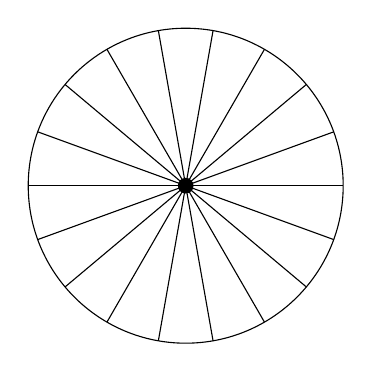
\begin{tikzpicture}
    \draw (0,0) circle (2cm);
    \foreach \x in {0,20,...,350}
      \draw[\OPTblue] (0,0) -- (\x:2cm);
    \node[\OPTblue,circle,fill,inner sep=2pt] (hub) at (0,0) {};
  \end{tikzpicture}
  \caption{由轮毂和辐条组成的 2-圆盘}
  \label{fig:hub-and-spokes}
\end{figure}

我们可以使用这个想法将包含 $n>1$ 维道路构造子的高阶归纳类型用只包含 1 维道路构造子的类型来表达。
关键是我们可以将 $n$ 维道路作为由 $(n-1)$ 维对象参数化的 1 维道路的连续族获得。
最简单的 $(n-1)$ 维对象是 $(n-1)$-球面,尽管在某些情况下可能更喜欢不同的对象。
(回想我们在\cref{sec:suspension}中能够使用悬挂归纳地定义球面,而悬挂只涉及 1 维道路构造子。
事实上,悬挂也可以看作是这个想法的一个实例,因为它涉及由被悬挂类型参数化的 1 维道路族。)

\index{torus}
例如,上一节的环面 $T^2$ 可以改为由以下构造子生成:
\begin{itemize}
\item 一个点 $b:T^2$,
\item 一条道路 $p:b=b$,
\item 另一条道路 $q:b=b$,
\item 一个点 $h:T^2$,以及
\item 对每个 $x:\Sn^1$,一条道路 $s(x) : f(x)=h$,其中 $f:\Sn^1\to T^2$ 由 $f(\base)\defeq b$ 和 $\ap f \lloop \defid p \ct q \ct \opp p \ct \opp q$ 定义。
\end{itemize}
这个版本的环面的归纳原理说给定 $P:T^2\to\type$,对于一个截面 $\prd{x:T^2} P(x)$,我们需要
\begin{itemize}
\item 一个点 $b':P(b)$,
\item 一条道路 $p' : \dpath P p {b'} {b'}$,
\item 一条道路 $q' : \dpath P q {b'} {b'}$,
\item 一个点 $h':P(h)$,以及
\item 对每个 $x:\Sn^1$,一条道路 $\dpath {P}{s(x)}{g(x)}{h'}$,其中 $g:\prd{x:\Sn^1} P(f(x))$ 由 $g(\base)\defeq b'$ 和 $\apd g \lloop \defid t(p' \ct q' \ct \opp{(p')} \ct \opp{(q')})$ 定义。
  在后者中,$\ct$ 表示依赖道路的串联,而 $t:\eqv{(\dpath{P}{\ap f \lloop}{b'}{b'})}{(\dpath{P\circ f}{\lloop}{b'}{b'})}$ 的定义留给读者。
\end{itemize}
注意不需要依赖 2-道路或 $\apdtwofunc{}$。
我们将计算规则的写出留给读者。

\begin{rmk}\label{rmk:spokes-no-hub}
人们可能会质疑引入轮毂点 $h$ 的必要性;为什么我们不能简单地添加道路,连续地将圆盘的边界关联到该边界\emph{上}的一点,如\cref{fig:spokes-no-hub}所示?
然而,这在没有进一步修改的情况下是行不通的。
因为如果给定某个 $f:\Sn^1 \to X$,我们给出一个道路构造子连接每个 $f(x)$ 到 $f(\base)$,那么我们最终得到的更像是\cref{fig:spokes-no-hub-ii}中的图片,一个锥的顶点被扭曲并粘贴到其底部的某点上。
问题是从 $f(\base)$ 到自身的指定道路可能不是自反性。
我们可以通过添加一个 2 维道路构造子来补救这个问题以确保这一点,但使用一个单独的轮毂避免了对维度高于 1 的任何道路构造子的需要。
\end{rmk}

\begin{figure}
  \centering
  \begin{minipage}{2in}
    \begin{center}
      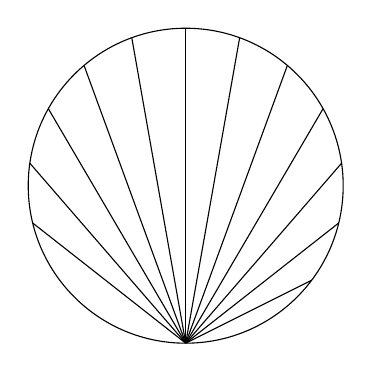
\begin{tikzpicture}
        \draw (0,0) circle (2cm);
        \clip (0,0) circle (2cm);
        \foreach \x in {0,15,...,165}
        \draw[\OPTblue] (0,-2cm) -- (\x:4cm);
      \end{tikzpicture}
    \end{center}
    \caption{无轮毂的辐条}
    \label{fig:spokes-no-hub}
  \end{minipage}
  \qquad
  \begin{minipage}{2in}
    \begin{center}
      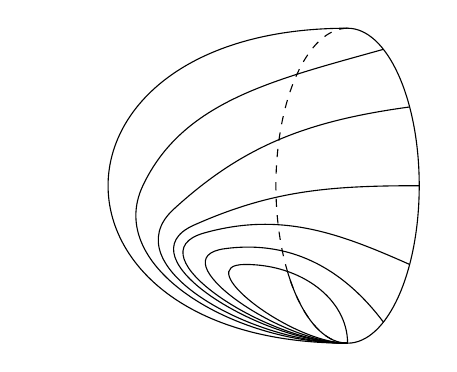
\begin{tikzpicture}[xscale=1.3]
        \draw (0,0) arc (-90:90:.7cm and 2cm) ;
        \draw[dashed] (0,4cm) arc (90:270:.7cm and 2cm) ;
        \draw[\OPTblue] (0,0) to[out=90,in=0] (-1,1) to[out=180,in=180] (0,0);
        \draw[\OPTblue] (0,4cm) to[out=180,in=180,looseness=2] (0,0);
        \path (0,0) arc (-90:-60:.7cm and 2cm) node (a) {};
        \draw[\OPTblue] (a.center) to[out=120,in=10] (-1.2,1.2) to[out=190,in=180] (0,0);
        \path (0,0) arc (-90:-30:.7cm and 2cm) node (b) {};
        \draw[\OPTblue] (b.center) to[out=150,in=20] (-1.4,1.4) to[out=200,in=180] (0,0);
        \path (0,0) arc (-90:0:.7cm and 2cm) node (c) {};
        \draw[\OPTblue] (c.center) to[out=180,in=30] (-1.5,1.5) to[out=210,in=180] (0,0);
        \path (0,0) arc (-90:30:.7cm and 2cm) node (d) {};
        \draw[\OPTblue] (d.center) to[out=190,in=50] (-1.7,1.7) to[out=230,in=180] (0,0);
        \path (0,0) arc (-90:60:.7cm and 2cm) node (e) {};
        \draw[\OPTblue] (e.center) to[out=200,in=70] (-2,2) to[out=250,in=180] (0,0);
        \clip (0,0) to[out=90,in=0] (-1,1) to[out=180,in=180] (0,0);
        \draw (0,4cm) arc (90:270:.7cm and 2cm) ;
      \end{tikzpicture}
    \end{center}
    \caption{无轮毂的辐条,II}
    \label{fig:spokes-no-hub-ii}
  \end{minipage}
\end{figure}

\begin{rmk}
  \index{computation rule!propositional}%
  还要注意,这种将高阶道路``翻译''为 1-道路的方式不保留这些道路的判断计算规则,尽管它确实保留命题计算规则。
\end{rmk}

\index{cell complex|)}%
\index{CW complex|)}%

\index{hub and spoke|)}%


\section{推出}
\label{sec:colimits}

\index{type!limit}%
\index{type!colimit}%
\index{limit!of types}%
\index{colimit!of types}%
从范畴论的角度来看,任何基础系统的重要方面之一是构造极限和余极限的能力。
在集合论基础中,这些是集合的极限和余极限,而在我们的情况下,它们是\emph{类型}的极限和余极限。
我们在\cref{sec:universal-properties}中看到笛卡尔积类型具有类型的范畴积的正确泛性质,在\cref{ex:coprod-ump}中看到余积类型同样具有其期望的泛性质。

如\cref{sec:universal-properties}中所述,更一般的极限可以使用恒等类型和 $\Sigma$-类型来构造,例如 $f:A\to C$ 和 $g:B\to C$ 的拉回\index{pullback}是 $\sm{a:A}{b:B} (f(a)=g(b))$(见\cref{ex:pullback})。
然而,更一般的\emph{余极限}需要等同来自不同类型的元素,高阶归纳类型非常适合这一点。
由于我们所有的构造都是同伦不变的,我们所有的余极限必然是\emph{同伦余极限},但为简洁起见,我们省略这个普遍的形容词。

在本节中,我们讨论\emph{推出},作为也许最简单和最有用的余极限之一。
事实上,人们期望所有有限余极限(对于``有限''的适当同伦定义)都可以从推出和有限余积构造。
也可以使用高阶归纳类型直接构造更一般的余极限,但这有些技术性,而且也不完全令人满意,因为我们还没有一个好的同伦相容图的完全一般概念。

\indexsee{type!pushout of}{pushout}%
\index{pushout|(defstyle}%
\index{span}%
假设给定类型和函数的跨越:
\[\Ddiag=\;\vcenter{\xymatrix{C \ar^g[r] \ar_f[d] & B \\ A & }}\]
这个跨越的\define{推出}是由以下呈现的高阶归纳类型 $A\sqcup^CB$:
\begin{itemize}
\item 一个函数 $\inl:A\to A\sqcup^CB$,
\item 一个函数 $\inr:B \to A\sqcup^CB$,以及
\item 对每个 $c:C$ 一条道路 $\glue(c):(\inl(f(c))=\inr(g(c)))$。
\end{itemize}
换言之,$A\sqcup^CB$ 是 $A$ 和 $B$ 的不相交并,连同对每个 $c:C$ 一个 $f(c)$ 和 $g(c)$ 相等的见证。
递归原理说如果 $D$ 是另一个类型,我们可以通过定义以下来定义映射 $s:A\sqcup^CB\to{}D$:
\begin{itemize}
\item 对每个 $a:A$,$s(\inl(a)):D$ 的值,
\item 对每个 $b:B$,$s(\inr(b)):D$ 的值,以及
\item 对每个 $c:C$,$\mapfunc{s}(\glue(c)):s(\inl(f(c)))=s(\inr(g(c)))$ 的值。
\end{itemize}
我们将归纳原理的表述留给读者。
它还蕴含唯一性原理,即如果 $s,s':A\sqcup^CB\to{}D$ 是两个映射使得
\index{uniqueness!principle, propositional!for functions on a pushout}%
\begin{align*}
  s(\inl(a))&=s'(\inl(a))\\
  s(\inr(b))&=s'(\inr(b))\\
  \mapfunc{s}(\glue(c))&=\mapfunc{s'}(\glue(c))
  \qquad\text{(模前两个等式)}
\end{align*}
对每个 $a,b,c$ 成立,则 $s=s'$。

为了表述推出的泛性质,我们引入以下定义。

\begin{defn}\label{defn:cocone}
  给定跨越 $\Ddiag= (A \xleftarrow{f} C \xrightarrow{g} B)$ 和类型 $D$,\define{顶点为 $D$ 的 $\Ddiag$ 下的余锥}
  \indexdef{cocone}%
  \index{vertex of a cocone}%
  由函数 $i:A\to{}D$ 和 $j:B\to{}D$ 以及同伦 $h : \prd{c:C} (i(f(c))=j(g(c)))$ 组成:
  \[\uppercurveobject{{ }}\lowercurveobject{{ }}\twocellhead{{ }}
  \xymatrix{C \ar^g[r] \ar_f[d] \drtwocell{^h} & B \ar^j[d] \\ A \ar_i[r] & D
  }\]
  我们用 $\cocone{\Ddiag}{D}$ 表示所有这类余锥的类型,即
  \[ \cocone{\Ddiag}{D} \defeq
  \sm{i:A\to D}{j:B\to D} \prd{c:C} (i(f(c))=j(g(c))).
  \]
\end{defn}

当然,存在顶点为 $A\sqcup^C B$ 的 $\Ddiag$ 下的一个典范余锥,由 $\inl$、$\inr$ 和 $\glue$ 组成。
\[\uppercurveobject{{ }}\lowercurveobject{{ }}\twocellhead{{ }}
\xymatrix{C \ar^g[r] \ar_f[d] \drtwocell{^\glue\ \ } & B \ar^\inr[d] \\
  A \ar_-\inl[r] & A\sqcup^CB }\]
以下引理说这是泛余锥。

\begin{lem}\label{thm:pushout-ump}
  \index{universal!property!of pushout}%
  对任意类型 $E$,存在等价
  \[ (A\sqcup^C B \to E) \;\eqvsym\; \cocone{\Ddiag}{E}. \]
\end{lem}
\begin{proof}
  考虑任意类型 $E:\type$。
  存在由以下定义的典范函数 $c_\sqcup$
  \[\function{(A\sqcup^CB\to{}E)}{\cocone{\Ddiag}{E}}
  {t}{(t\circ{}\inl,t\circ{}\inr,\mapfunc{t}\circ{}\glue)}\]
  我们非形式地将这个函数写作 $t\mapsto\composecocone{t}c_\sqcup$。
  我们证明这是一个等价。

  首先,给定 $c=(i,j,h):\cocone{\mathscr{D}}{E}$,我们需要构造一个从 $A\sqcup^CB$ 到 $E$ 的映射 $\mathsf{s}(c)$。
  \[\uppercurveobject{{ }}\lowercurveobject{{ }}\twocellhead{{ }}
  \xymatrix{C \ar^g[r] \ar_f[d] \drtwocell{^h} & B \ar^{j}[d] \\
    A \ar_-{i}[r] & E }\]
 映射 $\mathsf{s}(c)$ 以如下方式定义
  \begin{align*}
    \mathsf{s}(c)(\inl(a))&\defeq i(a),\\
    \mathsf{s}(c)(\inr(b))&\defeq j(b),\\
    \mapfunc{\mathsf{s}(c)}(\glue(x))&\defid h(x).
  \end{align*}
我们定义了映射
\[\function{\cocone{\Ddiag}{E}}{(A\sqcup^CB\to{}E)}{c}{\mathsf{s}(c)}\]
我们需要证明这个映射是 $t\mapsto{}\composecocone{t}c_\sqcup$ 的逆。
一方面,如果 $c=(i,j,h):\cocone{\Ddiag}{E}$,我们有
\begin{align*}
  \composecocone{\mathsf{s}(c)}c_\sqcup & =
  (\mathsf{s}(c)\circ\inl,\mathsf{s}(c)\circ\inr,
  \mapfunc{\mathsf{s}(c)}\circ\glue) \\
  & = (\lamu{a:A} \mathsf{s}(c)(\inl(a)),\;
  \lamu{b:B} \mathsf{s}(c)(\inr(b)),\;
  \lamu{x:C} \mapfunc{\mathsf{s}(c)}(\glue(x))) \\
  & = (\lamu{a:A} i(a),\;
  \lamu{b:B} j(b),\;
  \lamu{x:C} h(x)) \\
  & \jdeq (i, j, h) \\
  & = c.
\end{align*}
%
另一方面,如果 $t:A\sqcup^CB\to{}E$,我们想证明
$\mathsf{s}(\composecocone{t}c_\sqcup)=t$。
对 $a:A$,我们有
\[\mathsf{s}(\composecocone{t}c_\sqcup)(\inl(a))=t(\inl(a))\]
因为 $\composecocone{t}c_\sqcup$ 的第一个分量是 $t\circ\inl$。以同样的方式,对 $b:B$ 我们有
\[\mathsf{s}(\composecocone{t}c_\sqcup)(\inr(b))=t(\inr(b))\]
对 $x:C$ 我们有
\[\mapfunc{\mathsf{s}(\composecocone{t}c_\sqcup)}(\glue(x))
=\mapfunc{t}(\glue(x))\]
因此 $\mathsf{s}(\composecocone{t}c_\sqcup)=t$。

这证明了 $c\mapsto\mathsf{s}(c)$ 是 $t\mapsto{}\composecocone{t}c_\sqcup$ 的拟逆,如所需。
\end{proof}

许多标准的同伦论构造可以表示为(同伦)推出。
\begin{itemize}
\item 跨越 $\unit \leftarrow A \to \unit$ 的推出是\define{悬挂} $\susp A$(见\cref{sec:suspension})。%
  \index{suspension}
\symlabel{join}
\item $A \xleftarrow{\proj1} A\times B \xrightarrow{\proj2} B$ 的推出称为 $A$ 和 $B$ 的\define{连接},记作 $A*B$。%
  \indexdef{join!of types}
\item $\unit \leftarrow A \xrightarrow{f} B$ 的推出是 $f$ 的\define{锥}或\define{余纤维}。%
  \indexdef{cone!of a function}%
  \indexsee{mapping cone}{cone of a function}%
  \indexdef{cofiber of a function}%
\symlabel{wedge}
\item 如果 $A$ 和 $B$ 配备基点 $a_0:A$ 和 $b_0:B$,则 $A \xleftarrow{a_0} \unit \xrightarrow{b_0} B$ 的推出是\define{楔和} $A\vee B$。%
  \indexdef{wedge}
\symlabel{smash}
\item 如果 $A$ 和 $B$ 如前配备基点,定义 $f:A\vee B \to A\times B$,由 $f(\inl(a))\defeq (a,b_0)$ 和 $f(\inr(b))\defeq (a_0,b)$,以及 $\ap f \glue \defid \refl{(a_0,b_0)}$。
  则 $f$ 的锥称为\define{粉碎积} $A\wedge B$。%
  \indexdef{smash product}
\end{itemize}
我们将在\cref{cha:hlevels,cha:homotopy}中进一步讨论推出。

\begin{rmk}
  如\cref{subsec:prop-trunc}中所述,粉碎积和点型空间的楔和的记号 $\wedge$ 和 $\vee$ 也在逻辑中用于``与''和``或''。
  由于同伦类型论中的类型可以表现得像空间或像命题,因此技术上存在冲突的可能——但由于它们很少同时表现为两者,上下文通常能消歧义。
  此外,粉碎积和楔和只适用于\emph{点型}空间,而唯一的点型纯命题是 $\top\jdeq\unit$——且无论 $\wedge$ 和 $\vee$ 的哪种含义,我们都有 $\unit\wedge \unit = \unit$ 和 $\unit\vee\unit=\unit$。
\end{rmk}

\index{pushout|)}%

\begin{rmk}
  注意余极限一般不保持截断性。
  例如,$\Sn^0$ 和 \unit 都是集合,但 $\unit \leftarrow \Sn^0 \to \unit$ 的推出是 $\Sn^1$,它不是集合。
  如果我们对 $n$-类型范畴中的余极限感兴趣(特别是集合范畴),我们需要以某种方式``截断''余极限。
  我们将在\cref{sec:hittruncations,cha:hlevels,cha:set-math}中回到这一点。
\end{rmk}


\section{截断}
\label{sec:hittruncations}

\index{truncation!propositional|(}%
在\cref{subsec:prop-trunc}中,我们将命题截断引入为一种新的类型形成运算;
我们现在观察到它可以作为高阶归纳类型的特例获得。
这将理解截断的问题归约为理解高阶归纳类型的问题,后者至少可以系统地处理。
这也很有趣,因为它提供了我们第一个真正\emph{递归}的高阶归纳类型的例子,即其构造子的输入来自正在定义的类型(就像后继 $\suc:\nat\to\nat$ 一样)。

令 $A$ 是一个类型;我们将其命题截断 $\brck A$ 定义为由以下生成的高阶归纳类型:
\begin{itemize}
\item 一个函数 $\bprojf : A \to \brck A$,以及
\item 对每个 $x,y:\brck A$,一条道路 $x=y$。
\end{itemize}
注意第二个构造子根据定义就是断言 $\brck A$ 是纯命题。
因此,$\brck A$ 的定义可以解释为说 $\brck A$ 是由函数 $A\to\brck A$ 和它是纯命题的事实自由生成的。

这个高阶归纳定义的递归原理很容易写出:它说给定任意类型 $B$ 连同
\begin{itemize}
\item 一个函数 $g:A\to B$,以及
\item 对任意 $x,y:B$,一条道路 $x=_B y$,
\end{itemize}
存在函数 $f:\brck A \to B$ 使得
\begin{itemize}
\item 对所有 $a:A$ 有 $f(\bproj a) \jdeq g(a)$,以及
\item 对任意 $x,y:\brck A$,函数 $\apfunc f$ 将 $\brck A$ 中指定的道路 $x=y$ 映射到 $B$ 中指定的道路 $f(x) = f(y)$(命题地)。
\end{itemize}
\index{recursion principle!for truncation}%
这些正是我们在\cref{subsec:prop-trunc}中陈述的命题截断的递归原理的假设——一个函数 $A\to B$ 使得 $B$ 是纯命题——而结论的第一部分也正是我们在那里陈述的。
第二部分($\apfunc f$ 的作用)之前没有提到,但在这种情况下它实际上是空洞的,因为 $B$ 是纯命题,所以其中任意两条道路都自动相等。

\index{induction principle!for truncation}%
也有 $\brck A$ 的归纳原理,它说给定任意 $B:\brck A \to \type$ 连同
\begin{itemize}
\item 一个函数 $g:\prd{a:A} B(\bproj a)$,以及
\item 对任意 $x,y:\brck A$ 和 $u:B(x)$ 和 $v:B(y)$,一条依赖道路 $q:\dpath{B}{p(x,y)}{u}{v}$,其中 $p(x,y)$ 是来自 $\brck A$ 的第二个构造子的道路,
\end{itemize}
存在 $f:\prd{x:\brck A} B(x)$ 使得对 $a:A$ 有 $f(\bproj a)\jdeq g(a)$,以及另一个计算规则。
然而,由于任意两个纯命题之间最多有一个函数(在同伦意义下),这个归纳原理实际上不太有用(另见\cref{ex:prop-trunc-ind})。

\index{truncation!propositional|)}%
\index{truncation!set|(}%

\index{set|(}%
然而,我们可以扩展这个想法来构造类似的落入 $n$-类型的截断,对任意 $n$。
例如,我们可以定义\emph{0-截断} $\trunc0A$ 为由以下生成:
\begin{itemize}
\item 一个函数 $\tprojf0 : A \to \trunc0 A$,以及
\item 对每个 $x,y:\trunc0A$ 和每个 $p,q:x=y$,一条道路 $p=q$。
\end{itemize}
则 $\trunc0A$ 将由函数 $A\to \trunc0A$ 连同断言 $\trunc0A$ 是集合的事实自由生成。
其自然归纳原理将说给定 $B:\trunc0 A \to \type$ 连同
\begin{itemize}
\item 一个函数 $g:\prd{a:A} B(\tproj0a)$,以及
\item 对任意 $x,y:\trunc0A$ 配备 $z:B(x)$ 和 $w:B(y)$,以及每个 $p,q:x=y$ 配备 $r:\dpath{B}{p}{z}{w}$ 和 $s:\dpath{B}{q}{z}{w}$,一条 2-道路 $v:\dpath{\dpath{B}{-}{z}{w}}{u(x,y,p,q)}{r}{s}$,其中 $u(x,y,p,q):p=q$ 从 $\trunc0A$ 的第二个构造子获得,
\end{itemize}
存在 $f:\prd{x:\trunc0A} B(x)$ 使得对所有 $a:A$ 有 $f(\tproj0a)\jdeq g(a)$,以及 $\apdtwo{f}{u(x,y,p,q)}$ 是上面指定的 2-道路。
(如命题情况那样,后一个条件实际上是无趣的。)
然而,从此我们可以证明一个更有用的归纳原理。

\begin{lem}\label{thm:trunc0-ind}
  假设给定 $B:\trunc0 A \to \type$ 连同 $g:\prd{a:A} B(\tproj0a)$,并假设每个 $B(x)$ 是集合。
  则存在 $f:\prd{x:\trunc0A} B(x)$ 使得对所有 $a:A$ 有 $f(\tproj0a)\jdeq g(a)$。
\end{lem}
\begin{proof}
  只需对任意如上的 $x,y,z,w,p,q,r,s$ 构造一条 2-道路 $v:\dpath{B}{u(x,y,p,q)}{r}{s}$。
  然而,由依赖 2-道路的定义,这是纤维 $B(y)$ 中的普通 2-道路。
  由于 $B(y)$ 是集合,任意两条平行道路之间都存在 2-道路。
\end{proof}

这蕴含期望的泛性质。

\begin{lem}\label{thm:trunc0-lump}
  \index{universal!property!of truncation}%
  对任意集合 $B$ 和任意类型 $A$,与 $\tprojf0:A\to \trunc0A$ 的复合确定一个等价
  \[ \eqvspaced{(\trunc0A\to B)}{(A\to B)}. \]
\end{lem}
\begin{proof}
  当 $B$ 是常值族时,\cref{thm:trunc0-ind}的特例给出从右到左的映射,它是``与 $\tprojf0$ 复合''函数从左到右的右逆。
  要证明它也是左逆,令 $h:\trunc0A\to B$,并通过将\cref{thm:trunc0-ind}应用于复合 $a\mapsto h(\tproj0a)$ 定义 $h':\trunc0A\to B$。
  因此,$h'(\tproj0a)=h(\tproj0a)$。

  然而,由于 $B$ 是集合,对任意 $x:\trunc0A$,类型 $h(x)=h'(x)$ 是纯命题,因此也是集合。
  因此,由\cref{thm:trunc0-ind},对任意 $a:A$ 有 $h'(\tproj0a)=h(\tproj0a)$ 的观察蕴含对任意 $x:\trunc0A$ 有 $h(x)=h'(x)$,因此 $h=h'$。
\end{proof}

\index{limit!of sets}%
\index{colimit!of sets}%
例如,这使我们能够构造集合的余极限。
我们已经看到如果 $A \xleftarrow{f} C \xrightarrow{g} B$ 是集合的跨越,则推出 $A\sqcup^C B$ 可能不再是集合。
(例如,如果 $A$ 和 $B$ 是 \unit 而 $C$ 是 \bool,则推出是 $\Sn^1$。)
然而,我们可以通过截断构造一个是集合的推出,并对其他集合具有期望的泛性质。

\begin{lem}\label{thm:set-pushout}
  \index{universal!property!of pushout}%
  令 $A \xleftarrow{f} C \xrightarrow{g} B$ 是集合的跨越\index{span}。
  则对任意集合 $E$,存在典范等价
  \[ \Parens{\trunc0{A\sqcup^C B} \to E} \;\eqvsym\; \cocone{\Ddiag}{E}. \]
\end{lem}
\begin{proof}
  组合\cref{thm:pushout-ump,thm:trunc0-lump}中的等价。
\end{proof}

我们将 $\trunc0{A\sqcup^C B}$ 称为 $f$ 和 $g$ 的\define{集合-推出}
\indexdef{set-pushout}%
\index{pushout!of sets}
,以区别于(同伦)推出 $A\sqcup^C B$。
或者,我们可以修改\cref{sec:colimits}中推出的定义,直接包含 0-截断构造子,避免事后截断的需要。
类似的说明适用于任何类型的集合余极限;我们将在\cref{cha:set-math}中进一步探讨这一点。

然而,虽然上述 0-截断的定义有效——它给出我们想要的,并且是一致的——它有几个问题。
首先,它不太适合高阶归纳类型的一般理论。
一般来说,直接处理像我们为 $\trunc0A$ 给出的第二个那样的构造子是棘手的,其\emph{输入}不仅涉及正在定义的类型的元素,还涉及其中的道路。

然而,这可以相当容易地绕过。
回顾在\cref{sec:bool-nat}中我们提到,我们可以允许归纳类型 $W$ 的构造子通过让其接受类型为 $\nat\to W$ 的单个参数来接受 $W$ 类型的``无穷多个参数''。
这背后有一个一般原则:要建模具有奇怪输入的构造子,使用一个辅助归纳类型(如 \nat)来参数化它们,将输入归约为具有归纳定义域的简单函数。

对于 0-截断,我们可以考虑由两个点 $a,b:S$ 和两条道路 $p,q:a=b$ 生成的辅助\emph{高阶}归纳类型 $S$。
则 $\trunc 0A$ 的可疑构造子可以替换为无可厚非的
\begin{itemize}
\item 对每个 $f:S\to \trunc 0A$,一条道路 $\apfunc{f}(p) = \apfunc{f}(q)$。
\end{itemize}
由于给出从 $S$ 的映射等同于给出两点和它们之间的两条平行道路,这产生相同的归纳原理。

\index{set|)}%

\index{truncation!set|)}%
\index{truncation!n-truncation@$n$-truncation}%
然而,我们当前 0-截断定义的一个更严重的问题是它推广得不太好。
如果我们想对所有 $n:\nat$ 统一描述``$n$-截断''到 $n$-类型的定义概念,那么这种方法是不可行的,因为第二个构造子需要的参数数量随 $n$ 增加。
因此,在\cref{sec:truncations}中,我们将使用不同的想法来构造这些,基于上面引入的类型 $S$ 等价于圆周 $\Sn^1$ 的观察。
这包括 0-截断作为特例,并满足\cref{thm:trunc0-ind,thm:trunc0-lump}的推广版本。


\section{商}
\label{sec:set-quotients}

集合的一种特别重要的余极限是关于关系的\emph{商}。
即,令 $A$ 是集合且 $R:A\times A \to \prop$ 是纯命题族(一个\define{纯关系})。
\indexdef{relation!mere}%
\indexdef{mere relation}%
它的商应该是两个投影
\[ \tsm{a,b:A} R(a,b) \rightrightarrows A \]
的集合-等值化子。
我们也可以直接描述它,作为由以下生成的高阶归纳类型 $A/R$
\index{set-quotient|(defstyle}%
\indexsee{quotient of sets}{set-quotient}%
\indexsee{type!quotient}{set-quotient}%
\begin{itemize}
\item 一个函数 $q:A\to A/R$;
\item 对每个 $a,b:A$ 使得 $R(a,b)$,一个等式 $q(a)=q(b)$;以及
\item 0-截断构造子:对所有 $x,y:A/R$ 和 $r,s:x=y$,我们有 $r=s$。
\end{itemize}
我们有时将这个高阶归纳类型 $A/R$ 称为 $A$ 关于 $R$ 的\define{集合-商},以强调它根据定义产生一个集合。
(在同伦论中有更一般的``商''概念,但它们大多超出本书的范围。
然而,在\cref{sec:rezk}中我们将考虑类型关于 1-群胚的``商'',它是集合-商的上一层。)

\begin{rmk}\label{rmk:quotient-of-non-set}
  对于集合-商的定义及其大部分性质,实际上不需要 $A$ 是集合。
  然而,这通常是最感兴趣的情况。
\end{rmk}

\begin{lem}\label{thm:quotient-surjective}
  函数 $q:A\to A/R$ 是满射。
\end{lem}
\begin{proof}
  我们必须证明对任意 $x:A/R$ 纯粹存在 $a:A$ 使得 $q(a)=x$。
  我们使用 $A/R$ 的归纳原理。
  第一种情况是平凡的:如果 $x$ 是 $q(a)$,则当然纯粹存在 $a$ 使得 $q(a)=q(a)$。
  由于目标是纯命题,它自动遵守所有道路构造子,所以我们完成了。
\end{proof}

我们现在可以证明集合-商具有(集合-)等值化子的期望泛性质。

\begin{lem}\label{thm:quotient-ump}
  对任意集合 $B$,与 $q$ 预复合产生等价
  \[ \eqvspaced{(A/R \to B)}{\Parens{\sm{f:A\to B} \prd{a,b:A} R(a,b) \to (f(a)=f(b))}}.\]
\end{lem}
\begin{proof}
  $\blank\circ q$ 的拟逆,从右到左,就是 $A/R$ 的递归原理。
  即,给定 $f:A\to B$ 使得
  \narrowequation{\prd{a,b:A} R(a,b) \to (f(a)=f(b)),}
  我们定义 $\bar f:A/R\to B$,由 $\bar f(q(a))\defeq f(a)$。
  这个定义方程精确地说 $(f\mapsto \bar f)$ 是 $(\blank\circ q)$ 的右逆。

  为使它也是左逆,我们必须证明对任意 $g:A/R\to B$ 和 $x:A/R$ 有 $g(x) = \overline{g\circ q}(x)$。
  然而,由\cref{thm:quotient-surjective},纯粹存在 $a$ 使得 $q(a)=x$。
  由于我们想要的等式是纯命题,我们可以假设纯粹存在这样的 $a$,在这种情况下 $g(x) = g(q(a)) = \overline{g\circ q}(q(a)) = \overline{g\circ q}(x)$。
\end{proof}

当然,经典地通常考虑的情况是 $R$ 是\define{等价关系},即我们有
\indexdef{relation!equivalence}%
\indexsee{equivalence!relation}{relation, equivalence}%
%
\begin{itemize}
\item \define{自反性}:$\prd{a:A} R(a,a)$,
  \indexdef{reflexivity!of a relation}%
  \indexdef{relation!reflexive}%
\item \define{对称性}:$\prd{a,b:A} R(a,b) \to R(b,a)$,以及
  \indexdef{symmetry!of a relation}%
  \indexdef{relation!symmetric}%
\item \define{传递性}:$\prd{a,b,c:C} R(a,b) \times R(b,c) \to R(a,c)$。
  \indexdef{transitivity!of a relation}%
  \indexdef{relation!transitive}%
\end{itemize}
%
在这种情况下,集合-商 $A/R$ 有额外的好性质,我们将在\cref{sec:piw-pretopos}中看到:例如,我们有 $R(a,b) \eqvsym (\id[A/R]{q(a)}{q(b)})$。
\symlabel{equivalencerelation}
我们通常将等价关系 $R(a,b)$ 中缀地写作 $a\eqr b$。

等价关系的商也可以用其他方式构造。
集合论方法是将等价类的集合作为 $A$ 的幂集\index{power set}的子集来考虑。
我们也可以在类型论中模仿这种``非谓词''构造。
\index{impredicative!quotient}

\begin{defn}
  如果纯粹存在 $a:A$ 使得对所有 $b:A$ 有 $\eqv{R(a,b)}{P(b)}$,则谓词 $P:A\to\prop$ 是关系 $R : A \times A \to \prop$ 的\define{等价类}。
  \indexdef{equivalence!class}%
\end{defn}

由于 $R$ 和 $P$ 是纯命题,等价 $\eqv{R(a,b)}{P(b)}$ 等同于蕴含 $R(a,b) \to P(b)$ 和 $P(b) \to R(a,b)$。
当然,对任意 $a:A$ 我们有典范等价类 $P_a(b) \defeq R(a,b)$。

\begin{defn}\label{def:VVquotient}
  我们定义
  \begin{equation*}
    A\sslash R \defeq \setof{ P:A\to\prop | P \text{ 是 } R \text{ 的等价类}}.
  \end{equation*}
  函数 $q':A\to A\sslash R$ 由 $q'(a) \defeq P_a$ 定义。
\end{defn}

\begin{thm}
  对任意 $A$ 上的等价关系 $R$,类型 $A\sslash R$ 等价于集合-商 $A/R$。
\end{thm}
\begin{proof}
  首先,注意如果 $R(a,b)$,则由于 $R$ 是等价关系,对任意 $c:A$ 有 $R(a,c) \Leftrightarrow R(b,c)$。
  因此,由泛等性有 $R(a,c) = R(b,c)$,由函数外延性有 $P_a=P_b$,即 $q'(a)=q'(b)$。
  因此,由\cref{thm:quotient-ump}我们有诱导映射 $f:A/R \to A\sslash R$ 使得 $f\circ q = q'$。

  我们证明 $f$ 是单射和满射,因此是等价。
  满射性直接由 $q'$ 是满射的事实得出,这又基本上由 $A\sslash R$ 的定义为真。
  对于单射性,如果 $f(x)=f(y)$,则要证明纯命题 $x=y$,由 $q$ 的满射性我们可以假设 $x=q(a)$ 且 $y=q(b)$ 对某些 $a,b:A$。
  则对任意 $c:A$ 有 $R(a,c) = f(q(a))(c) = f(q(b))(c) = R(b,c)$,特别地 $R(a,b) = R(b,b)$。
  但 $R(b,b)$ 是有居民的,因为 $R$ 是等价关系,因此 $R(a,b)$ 也是。
  因此 $q(a)=q(b)$,所以 $x=y$。
\end{proof}

在\cref{subsec:quotients}中,我们将给出这个定理的另一个证明。
注意与 $A/R$ 不同,构造 $A\sslash R$ 提升宇宙层级:如果 $A:\UU_i$ 且 $R:A\to A\to \prop_{\UU_i}$,则在 $A\sslash R$ 的定义中我们也必须使用 $\prop_{\UU_i}$ 来包含所有等价类,使得 $A\sslash R : \UU_{i+1}$。
当然,如果我们假设\cref{subsec:prop-subsets}中的命题重整大小公理,我们可以避免这一点。

\begin{rmk}\label{defn-Z}
前两个构造提供了一般性的商,但在特定情况下可能有更简单的构造。
例如,我们可以将整数 \Z 定义为集合-商
\indexdef{integers}%
\indexdef{number!integers}%
%
\[ \Z \defeq (\N \times \N)/{\eqr} \]
%
其中 $\eqr$ 是由
%
\[ (a,b) \eqr (c,d) \defeq (a + d = b + c) \]
%
定义的等价关系。
换言之,一对 $(a,b)$ 表示整数 $a - b$。
然而,在这种情况下,等价类有\emph{典范代表}:形如 $(n,0)$ 或 $(0,n)$ 的那些。
\end{rmk}

以下引理说当这类事情发生时,我们不需要任何一般的商构造。
(函数 $r:A\to A$ 称为\define{幂等的}
\indexdef{function!idempotent}%
\indexdef{idempotent!function}%
如果 $r\circ r = r$。)

\begin{lem}\label{lem:quotient-when-canonical-representatives}
  假设 $\eqr$ 是集合 $A$ 上的关系,且存在幂等函数 $r : A \to A$ 使得对所有 $x, y: A$ 有 $\eqv{(r(x) = r(y))}{(x \eqr y)}$。
  (这蕴含 $\eqr$ 是等价关系。)
  则类型
  %
  \begin{equation*}
    (A/{\eqr}) \defeq \Parens{\sm{x : A} r(x) = x}
  \end{equation*}
  %
  满足 $A$ 关于 $\eqr$ 的集合-商的泛性质,因此与之等价。
  换言之,存在映射 $q : A \to (A/{\eqr})$ 使得对每个集合 $B$,与 $q$ 预复合诱导等价
  %
  \begin{equation}
    \label{eq:quotient-when-canonical}
    \Parens{(A/{\eqr}) \to B} \eqvsym \Parens{\sm{g : A \to B} \prd{x, y : A} (x \eqr y) \to (g(x) = g(y))}.
  \end{equation}
\end{lem}

\begin{proof}
  令 $i : \prd{x : A} r(r(x)) = r(x)$ 见证 $r$ 的幂等性。
  映射 $q : A \to (A/{\eqr})$ 由 $q(x) \defeq (r(x), i(x))$ 定义。
  注意由于 $A$ 是集合,我们有 $q(x)=q(y)$ 当且仅当 $r(x)=r(y)$,因此(由假设)当且仅当 $x \eqr y$。
  我们定义\eqref{eq:quotient-when-canonical}中从左到右的映射 $e$,由
  \[ e(f) \defeq (f \circ q, \nameless), \]
  %
  其中下划线 $\nameless$ 表示以下证明:如果 $x, y : A$ 且 $x \eqr y$,则如上所述 $q(x)=q(y)$,因此 $f(q(x)) = f(q(y))$。
  要看出 $e$ 是等价,考虑反方向的映射 $e'$,定义为
  %
  \[ e'(g, s) (x,p) \defeq g(x). \]
  %
  给定任意 $f : (A/{\eqr}) \to B$,
  %
  \[ e'(e(f))(x, p) \jdeq f(q(x)) \jdeq f(r(x), i(x)) = f(x, p) \]
  %
  其中最后一个等式成立因为 $p : r(x) = x$,所以 $(x,p) = (r(x), i(x))$,因为 $A$ 是集合。类似地我们计算
  %
  \[ e(e'(g, s)) \jdeq e(g \circ \proj{1}) \jdeq (g \circ \proj{1} \circ q, {\nameless}). \]
  %
  由于 $B$ 是集合,我们不需要担心 $\nameless$ 部分,而对于第一个分量我们有
  %
  \[ g(\proj{1}(q(x))) \jdeq g(r(x)) = g(x), \]
  %
  其中最后一个方程成立因为 $r(x) \eqr x$,而 $g$ 由假设 $s$ 遵守 $\eqr$。
\end{proof}

\begin{cor}\label{thm:retraction-quotient}
  假设 $p:A\to B$ 是集合之间的收缩。
  则 $B$ 是 $A$ 关于由
  \[ (a_1 \eqr a_2) \defeq (p(a_1) = p(a_2)) \]
  定义的等价关系 $\eqr$ 的商。
\end{cor}
\begin{proof}
  假设 $s:B\to A$ 是 $p$ 的截面。
  则 $s\circ p : A\to A$ 是满足\cref{lem:quotient-when-canonical-representatives}对这个 $\eqr$ 的条件的幂等函数,而 $s$ 诱导从 $B$ 到其不动点集的同构。
\end{proof}

\begin{rmk}\label{Z-quotient-by-canonical-representatives}
\cref{lem:quotient-when-canonical-representatives}应用于 \Z,配备由
%
\begin{equation*}
  r(a, b) =
  \begin{cases}
    (a - b, 0) & \text{如果 $a \geq b$,} \\
    (0, b - a) & \text{否则}
  \end{cases}
\end{equation*}
%
定义的幂等函数 $r : \N \times \N \to \N \times \N$。
(即使构造性地这也是有效的定义,因为 $\N$ 上的关系 $\geq$ 是可判定的。)
因此非负整数典范地表示为 $(k, 0)$,非正整数表示为 $(0, m)$,对 $k,m:\N$。
这种情况划分蕴含以下整数的``归纳原理'',它将在\cref{cha:homotopy}中有用。
\index{natural numbers}%
(像往常一样,我们将自然数 $n$ 与相应的非负整数等同,即 $\N\times\N$ 中 $(n,0)$ 在 $\Z$ 中的像。)
\end{rmk}

\begin{lem}\label{thm:sign-induction}
  \index{integers!induction principle for}%
  \index{induction principle!for integers}%
  假设 $P:\Z\to\type$ 是类型族且我们有
  \begin{itemize}
  \item $d_0: P(0)$,
  \item $d_+: \prd{n:\N} P(n) \to P(\suc(n))$,以及
  \item $d_- : \prd{n:\N} P(-n) \to P(-\suc(n))$。
  \end{itemize}
  则我们有 $f:\prd{z:\Z} P(z)$ 使得
  \begin{itemize}
    \item $f(0) = d_0$,
    \item 对所有 $n:\N$ 有 $f(\suc(n)) = d_+(n,f(n))$,以及
    \item 对所有 $n:\N$ 有 $f(-\suc(n)) = d_-(n,f(-n))$。
  \end{itemize}
\end{lem}
\begin{proof}
  为了这个证明,令 $\Z$ 表示 $\sm{x:\N\times\N}(r(x)=x)$,其中 $r$ 是上述幂等函数。
  (我们可以将结果传输到任何等价的 $\Z$ 定义。)
  令 $q:\N\times\N\to\Z$ 是商映射,由\cref{lem:quotient-when-canonical-representatives}中的 $q(x) = (r(x),i(x))$ 定义。
  现在定义 $Q\defeq P\circ q:\N\times \N \to \type$。
  通过将给定数据跨越适当的等式传输,我们得到
  \begin{align*}
    d'_0 &: Q(0,0)\\
    d'_+ &: \prd{n:\N} Q(n,0) \to Q(\suc(n),0)\\
    d'_- &: \prd{n:\N} Q(0,n) \to Q(0,\suc(n)).
  \end{align*}
  还要注意由于 $q(n,m) = q(\suc(n),\suc(m))$,我们有诱导等价
  \[e_{n,m}:\eqv{Q(n,m)}{Q(\suc(n),\suc(m))}.\]
  我们然后可以通过对 $x$ 的双重归纳构造 $g:\prd{x:\N\times \N} Q(x)$:
  \begin{align*}
    g(0,0) &\defeq d'_0,\\
    g(\suc(n),0) &\defeq d'_+(n,g(n,0)),\\
    g(0,\suc(m)) &\defeq d'_-(m,g(0,m)),\\
    g(\suc(n),\suc(m)) &\defeq e_{n,m}(g(n,m)).
  \end{align*}
  现在我们有 $\proj1 : \Z \to \N\times\N$,具有性质 $q\circ \proj1 = \idfunc$。
  特别地,因此我们有 $Q\circ \proj1 = P$,从而有等价族 $s:\prd{z:\Z} \eqv{Q(\proj1(z))}{P(z)}$。
  因此,我们可以定义 $f(z) = s(z,g(\proj1(z)))$ 得到 $f:\prd{z:\Z} P(z)$,并验证期望的等式。
\end{proof}

我们有时用模式匹配语法表示由\cref{thm:sign-induction}得到的函数 $f:\prd{z:\Z} P(z)$,涉及三种情况 $d_0$、$d_+$ 和 $d_-$:
\begin{align*}
  f(0) &\defid d_0\\
  f(\suc(n)) &\defid d_+(n,f(n))\\
  f(-\suc(n)) &\defid d_-(n,f(-n))
\end{align*}
我们使用 $\defid$ 而不是 $\defeq$,就像我们对高阶归纳类型的道路构造子所做的那样,以表明\cref{thm:sign-induction}蕴含的``计算''规则只是命题等式。
例如,以这种方式我们可以为任意整数 $n$ 定义环路的 $n$ 重串联。

\begin{cor}\label{thm:looptothe}
  \indexdef{path!concatenation!n-fold@$n$-fold}%
  令 $A$ 是类型,配备 $a:A$ 和 $p:a=a$。
  存在函数 $\prd{n:\Z} (a=a)$,记作 $n\mapsto p^n$,定义为
  \begin{align*}
    p^0 &\defid \refl{a}\\
    p^{n+1} &\defid p^n \ct p
    & &\text{对 $n\ge 0$}\\
    p^{n-1} &\defid p^n \ct \opp p
    & &\text{对 $n\le 0$。}
  \end{align*}
\end{cor}

我们将在\cref{sec:free-algebras,sec:field-rati-numb}中进一步讨论整数。

\index{set-quotient|)}%

\section{代数}
\label{sec:free-algebras}

除了构造像球面和胞腔复形这样的高维对象外,即使只处理集合,高阶归纳类型也非常有用。
我们已经在\cref{thm:set-pushout}中看到一个例子:它们允许我们构造任何集合图的余极限,这在\cref{cha:typetheory}的基本类型论中是不可能的。
当我们研究具有代数结构的集合时,高阶归纳类型也非常有用。

作为本节的运行例子,我们考虑\emph{群},它对大多数数学家来说是熟悉的,并展示了基本现象(且在后面的章节中会需要)。
然而,我们所说的大部分同样适用于任何类型的代数结构。

\index{monoid|(}%

\begin{defn}
  \define{幺半群}
  \indexdef{monoid}%
  是集合 $G$ 配备
  \begin{itemize}
  \item 一个\emph{乘法}
    \indexdef{multiplication!in a monoid}%
    \indexdef{multiplication!in a group}%
    函数 $G\times G\to G$,中缀地写作 $(x,y) \mapsto x\cdot y$;以及
  \item 一个\emph{单位}
    \indexdef{unit!of a monoid}%
    \indexdef{unit!of a group}%
    元素 $e:G$;使得
  \item 对任意 $x:G$,有 $x\cdot e = x$ 且 $e\cdot x = x$;以及
  \item 对任意 $x,y,z:G$,有 $x\cdot (y\cdot z) = (x\cdot y)\cdot z$。
    \index{associativity!in a monoid}%
    \index{associativity!in a group}%
  \end{itemize}
  \define{群}
  \indexdef{group}%
  是幺半群 $G$ 配备
  \begin{itemize}
  \item 一个\emph{逆}函数 $i:G\to G$,写作 $x\mapsto \opp x$;使得
    \index{inverse!in a group}%
  \item 对任意 $x:G$ 有 $x\cdot \opp x = e$ 且 $\opp x \cdot x = e$。
  \end{itemize}
\end{defn}

\begin{rmk}\label{rmk:infty-group}
注意我们要求群是集合。
我们可以考虑不是集合的更一般的``$\infty$-群''%
\index{.infinity-group@$\infty$-group}
概念,但这会把我们带得比目前合适的更远。
用我们目前的定义,我们可以期望得到的``群论''与它在集合论数学中的行为类似(需要注意的是,除非我们假设\LEM{},它将是``构造性''群论)。\index{mathematics!constructive}
\end{rmk}

\begin{eg}
  自然数 \N 在加法下是幺半群,单位为 $0$,在乘法下也是幺半群,单位为 $1$。
  如果我们以明显的方式定义整数 \Z 上的算术运算,则像往常一样它们在加法下是群,在乘法下是幺半群(当然,还是环)。
  例如,如果 $u, v \in \Z$ 分别由 $(a,b)$ 和 $(c,d)$ 表示,则 $u + v$ 由 $(a + c, b + d)$ 表示,$-u$ 由 $(b, a)$ 表示,$u v$ 由 $(a c + b d, a d + b c)$ 表示。
\end{eg}

\begin{eg}\label{thm:homotopy-groups}
  我们本质上在\cref{sec:equality}中观察到,如果 $(A,a)$ 是点型类型,则其环路空间\index{loop space} $\Omega(A,a)\defeq (\id[A]aa)$ 具有群的所有结构,除了它一般不是集合。
  它应该是\cref{rmk:infty-group}中提到意义上的``$\infty$-群'',但我们也可以通过截断使它成为群。
  具体地,我们定义 $A$ 在 $a:A$ 处的\define{基本群}
  \indexsee{group!fundamental}{fundamental group}%
  \indexdef{fundamental!group}%
  为
  \[\pi_1(A,a)\defeq \trunc0{\Omega(A,a)}.\]
  这继承了群结构;例如,乘法 $\pi_1(A,a) \times \pi_1(A,a) \to \pi_1(A,a)$ 由对截断的双重归纳从道路串联定义。

  更一般地,$(A,a)$ 的\define{第 $n$ 同伦群}
  \index{homotopy!group}%
  \indexsee{group!homotopy}{homotopy group}%
  是 $\pi_n(A,a)\defeq \trunc0{\Omega^n(A,a)}$。
  \index{loop space!iterated}%
  则对 $n\ge 1$ 有 $\pi_n(A,a) = \pi_1(\Omega^{n-1}(A,a))$,所以它也是群。
  (当 $n=0$ 时,我们有 $\pi_0(A) \jdeq \trunc0 A$,它不是群。)
  此外,Eckmann--Hilton 论证\index{Eckmann--Hilton argument}(\cref{thm:EckmannHilton})蕴含如果 $n\ge 2$,则 $\pi_n(A,a)$ 是\emph{阿贝尔}\index{group!abelian}群,即对所有 $x,y$ 有 $x\cdot y = y\cdot x$。
  \cref{cha:homotopy}将主要是对这些群的研究。
\end{eg}

\index{algebra!free}%
\index{free!algebraic structure}%
群论中的一个重要概念是由集合生成的\emph{自由群},或更一般地由生成元\index{generator!of a group}和关系\emph{表示}的群。
在类型论中众所周知,\emph{某些}自由代数对象可以使用\emph{普通}归纳类型定义。
\symlabel{lst-freemonoid}%
\indexdef{type!of lists}%
\indexsee{list type}{type, of lists}%
\index{monoid!free|(}%
例如,集合 $A$ 上的自由幺半群可以与 $A$ 的元素的\emph{有限列表}\index{finite!lists, type of}类型 $\lst A$ 等同,它由以下归纳生成:
\begin{itemize}
\item 一个构造子 $\nil:\lst A$,以及
\item 对每个 $\ell:\lst A$ 和 $a:A$,一个元素 $\cons(a,\ell):\lst A$。
\end{itemize}
我们有明显的包含 $\eta : A\to \lst A$,由 $a\mapsto \cons(a,\nil)$ 定义。
$\lst A$ 上的幺半群运算是串联,递归地定义为
\begin{align*}
  \nil \cdot \ell &\defeq \ell\\
  \cons (a,\ell_1) \cdot \ell_2 &\defeq \cons(a, \ell_1\cdot\ell_2).
\end{align*}
使用 $\lst A$ 的归纳原理,证明 $\lst A$ 是集合且列表串联是结合的
\index{associativity!of list concatenation}%
且以 $\nil$ 为单位是直接的。
因此,$\lst A$ 是幺半群。

\begin{lem}\label{thm:free-monoid}
  \indexsee{free!monoid}{monoid, free}%
  对任意集合 $A$,类型 $\lst A$ 是 $A$ 上的自由幺半群。
  换言之,对任意幺半群 $G$,与 $\eta$ 的复合是等价
  \[ \eqv{\hom_{\mathrm{Monoid}}(\lst A,G)}{(A\to G)}, \]
  其中 $\hom_{\mathrm{Monoid}}(\blank,\blank)$ 表示幺半群同态(保持乘法和单位的函数)的集合。
  \indexdef{homomorphism!monoid}%
  \indexdef{monoid!homomorphism}%
\end{lem}
\begin{proof}
  给定 $f:A\to G$,我们递归地定义 $\bar{f}:\lst A \to G$:
  \begin{align*}
    \bar{f}(\nil) &\defeq e\\
    \bar{f}(\cons(a,\ell)) &\defeq f(a) \cdot \bar{f}(\ell).
  \end{align*}
  通过归纳直接证明 $\bar{f}$ 是幺半群同态,且 $f\mapsto \bar f$ 是 $(\blank\circ \eta)$ 的拟逆;见\cref{ex:free-monoid}。
\end{proof}

\index{monoid!free|)}%

这种自由幺半群的构造之所以可能,本质上是因为自由幺半群的元素有可计算的典范形式(即有限列表)。
然而,其他自由(和表示的)代数结构——如群——的元素一般没有\emph{可计算的}典范形式。
例如,群表示中的字等价性是算法上\index{algorithm}不可判定的。
然而,我们仍然可以将自由代数对象描述为\emph{高阶}归纳类型,通过简单地将所有公理方程断言为道路构造子。

\indexsee{free!group}{group, free}%
\index{group!free|(}%
例如,令 $A$ 是集合,并定义高阶归纳类型 $\freegroup{A}$ 具有以下生成元。
\begin{itemize}
\item 一个函数 $\eta:A\to \freegroup{A}$。
\item 一个函数 $m: \freegroup{A} \times \freegroup{A} \to \freegroup{A}$。
\item 一个元素 $e:\freegroup{A}$。
\item 一个函数 $i:\freegroup{A} \to \freegroup{A}$。
\item 对每个 $x,y,z:\freegroup{A}$,一个等式 $m(x,m(y,z)) = m(m(x,y),z)$。
\item 对每个 $x:\freegroup{A}$,等式 $m(x,e) = x$ 和 $m(e,x) = x$。
\item 对每个 $x:\freegroup{A}$,等式 $m(x,i(x)) = e$ 和 $m(i(x),x) = e$。
\item 0-截断构造子:对任意 $x,y:\freegroup{A}$ 和 $p,q:x=y$,有 $p=q$。
\end{itemize}
第一个构造子说 $A$ 映射到 $\freegroup{A}$。
接下来三个给 $\freegroup{A}$ 群的运算:乘法、单位元和逆。
之后三个构造子断言群的公理:结合律\index{associativity}、单位性和逆。
最后,最后一个构造子断言 $\freegroup{A}$ 是集合。

因此,$\freegroup{A}$ 是群。
以下也是直接证明的:

\begin{thm}
  \index{universal!property!of free group}%
  $\freegroup{A}$ 是 $A$ 上的自由群。
  换言之,对任意(集合)群 $G$,与 $\eta:A\to \freegroup{A}$ 的复合确定等价
  \[ \hom_{\mathrm{Group}}(\freegroup{A},G) \eqvsym (A\to G) \]
  其中 $\hom_{\mathrm{Group}}(\blank,\blank)$ 表示两个群之间群同态的集合。
  \indexdef{group!homomorphism}%
  \indexdef{homomorphism!group}%
\end{thm}
\begin{proof}
  高阶归纳类型 $\freegroup{A}$ 的递归原理\emph{精确地}说如果 $G$ 是群且我们有 $f:A\to G$,则有 $\bar{f}:\freegroup{A} \to G$。
  它的计算规则说 $\bar{f}\circ \eta \jdeq f$,且 $\bar f$ 是群同态。
  因此,$(\blank\circ \eta) :  \hom_{\mathrm{Group}}(\freegroup{A},G) \to (A\to G)$ 有右逆。
  使用 $\freegroup{A}$ 的归纳原理直接证明这也是左逆。
\end{proof}

\index{acceptance}
值得退后一步考虑我们刚才做了什么。
我们\emph{没有}给出任何集合上的自由群的显式构造就证明了它的存在。
本质上我们只需写下它应该满足的泛性质。
在集合论中,我们可以通过诉诸伴随函子定理\index{adjoint!functor theorem}这样的黑箱来实现类似的结果;类型论将这类构造建入数学的基础。

当然,有时具体描述自由代数结构也是有用的。
对于自由群,我们可以使用商提供一个。
考虑 $\lst{A+A}$,其中在 $A+A$ 中我们将 $\inl(a)$ 写作 $a$,$\inr(a)$ 写作 $\hat{a}$(意在代表 $a$ 的形式逆)。
$\lst{A+A}$ 的元素是 $A$ 上自由群的\emph{字}。

\begin{thm}
  令 $A$ 是集合,令 $\freegroupx{A}$ 是 $\lst{A+A}$ 关于以下关系的集合-商。
  \begin{align*}
    (\dots,a_1,a_2,\widehat{a_2},a_3,\dots) &=
    (\dots,a_1,a_3,\dots)\\
    (\dots,a_1,\widehat{a_2},a_2,a_3,\dots) &=
    (\dots,a_1,a_3,\dots).
  \end{align*}
  则 $\freegroupx{A}$ 也是集合 $A$ 上的自由群。
\end{thm}
\begin{proof}
  首先我们证明 $\freegroupx{A}$ 是群。
  我们已经看到 $\lst{A+A}$ 是幺半群;我们声称幺半群结构下降到商。
  我们通过双重商递归定义 $\freegroupx{A} \times \freegroupx{A} \to \freegroupx{A}$;只需检查由给定关系生成的等价关系在列表串联下保持。
  类似地,我们通过商归纳证明结合律和单位律。

  为了在 $\freegroupx{A}$ 中定义逆,我们首先通过列表递归定义 $\mathsf{reverse}:\lst B\to\lst B$:
  \begin{align*}
    \mathsf{reverse}(\nil) &\defeq \nil,\\
    \mathsf{reverse}(\cons(b,\ell))&\defeq \mathsf{reverse}(\ell)\cdot \cons(b,\nil).
  \end{align*}
  现在我们通过商递归定义 $i:\freegroupx{A}\to \freegroupx{A}$,作用于列表 $\ell:\lst{A+A}$ 时交换 $A$ 的两个副本并反转列表。
  这保持关系,因此下降到商。
  我们可以通过归纳证明对 $x:\freegroupx{A}$ 有 $i(x) \cdot x = e$。
  首先,商归纳允许我们假设 $x$ 来自 $\ell:\lst{A+A}$,然后我们可以做列表归纳;如果我们将商映射写作 $q:\lst{A+A}\to \freegroupx{A}$,情况是
  \begin{align*}
    i(q(\nil)) \ct q(\nil) &= q(\nil) \ct q(\nil)\\
    &= q(\nil)\\
    i(q(\cons(a,\ell))) \ct q(\cons(a,\ell)) &= i(q(\ell)) \ct q(\cons(\hat{a},\nil)) \ct q(\cons(a,\ell))\\
    &= i(q(\ell)) \ct q(\cons(\hat{a},\cons(a,\ell)))\\
    &= i(q(\ell)) \ct q(\ell)\\
    &= q(\nil). \tag{由归纳假设}
  \end{align*}
  (我们省略了一些关于列表串联行为等的相当明显的引理。)

  这完成了 $\freegroupx{A}$ 是群的证明。
  现在如果 $G$ 是任意群,配备函数 $f:A\to G$,我们可以定义 $A+A\to G$ 为在 $A$ 的第一个副本上是 $f$,在第二个副本上是 $f$ 与 $G$ 的逆映射的复合。
  现在 $G$ 是幺半群的事实产生幺半群同态 $\lst{A+A} \to G$。
  由于 $G$ 是群,这个映射遵守关系,因此下降到映射 $\freegroupx{A}\to G$。
  直接证明这是群同态,且是限制到 $A$ 上为 $f$ 的唯一这样的同态。
\end{proof}

\index{monoid|)}%

如果 $A$ 有可判定等式\index{decidable!equality}(例如如果我们假设排中律),则定义 $\freegroupx{A}$ 的商可以像\cref{lem:quotient-when-canonical-representatives}中那样从幂等函数获得。
我们定义一个字,我们回顾它只是 $\lst{A+A}$ 的元素,如果它不包含形如 $(a,\hat a)$ 或 $(\hat a,a)$ 的相邻对,则称为\define{约化的}
\indexdef{reduced word in a free group}
。
当 $A$ 有可判定等式时,定义字的\define{约化}
\index{reduction!of a word in a free group}%
是直接的,它是生成适当商的幂等函数;我们将细节留给读者。

如果 $A\defeq \unit$,它有可判定等式,约化的字必须完全由 $\ttt$ 组成或完全由 $\hat{\ttt}$ 组成。
因此,$\unit$ 上的自由群等价于整数 \Z,其中 $0$ 对应于 $\nil$,正整数 $n$ 对应于 $n$ 个 $\ttt$ 的约化字,负整数 $(-n)$ 对应于 $n$ 个 $\hat{\ttt}$ 的约化字。
当然,也可以直接证明 \Z 具有 $\freegroup{\unit}$ 的泛性质。

\begin{rmk}\label{thm:freegroup-nonset}
  在 $\freegroup{A}$ 和 $\freegroupx{A}$ 的构造及其泛性质的证明中,我们没有在任何地方使用 $A$ 是集合的假设。
  因此,我们实际上可以构造任意类型上的自由群。
  比较泛性质,我们得出 $\eqv{\freegroup{A}}{\freegroup{\trunc0A}}$。
\end{rmk}

\index{group!free|)}%

\index{algebra!colimits of}%
我们也可以使用高阶归纳类型来构造代数对象的余极限。
例如,假设 $f:G\to H$ 和 $g:G\to K$ 是群同态。
它们在群范畴中的推出,称为\define{合并自由积}
\indexdef{amalgamated free product}%
\indexdef{free!product!amalgamated}%
$H *_G K$,可以构造为由以下生成的高阶归纳类型:
\begin{itemize}
\item 函数 $h:H\to H *_G K$ 和 $k:K\to H *_G K$。
\item 群的运算和公理,如 $\freegroup{A}$ 的定义中那样。
\item 断言 $h$ 和 $k$ 是群同态的公理。
\item 对 $x:G$,我们有 $h(f(x)) = k(g(x))$。
\item 0-截断构造子。
\end{itemize}
另一方面,它也可以显式构造为 $\lst{H+K}$ 关于以下关系的集合-商:
\begin{align*}
  (\dots, x_1, x_2, \dots) &= (\dots, x_1\cdot x_2, \dots)
  & &\text{对 $x_1,x_2:H$}\\
  (\dots, y_1, y_2, \dots) &= (\dots, y_1\cdot y_2, \dots)
  & &\text{对 $y_1,y_2:K$}\\
  (\dots, 1_G, \dots) &= (\dots, \dots) &&  \\
  (\dots, 1_H, \dots) &= (\dots, \dots) &&  \\
  (\dots, f(x), \dots) &= (\dots, g(x), \dots)
  & &\text{对 $x:G$。}
\end{align*}
我们将证明留给读者。
在 $G$ 是平凡群的特殊情况下,最后一个关系是不必要的,我们得到\define{自由积}
\indexdef{free!product}%
$H*K$,群范畴中的余积。
(这个记号不幸地与\cref{sec:colimits}中类型的\emph{连接}的记号冲突,但上下文通常能消歧义。)

\index{presentation!of a group}%
注意由\emph{表示}定义的群可以看作是余极限的特例。
假设给定集合(或更一般地类型)$A$,和一对函数 $R\rightrightarrows \freegroup{A}$。
我们将 $R$ 视为``关系''的类型,两个函数将每个关系分配给它使相等的两个字。
例如,在表示 $\langle a \mid a^2 = e \rangle$ 中,我们将有 $A\defeq \unit$ 和 $R\defeq \unit$,两个态射 $R\rightrightarrows \freegroup{A}$ 分别选出列表 $(a,a)$ 和空列表 $\nil$。
然后由自由群的泛性质,我们得到一对群同态 $\freegroup{R} \rightrightarrows \freegroup{A}$。
它们在群范畴中的等值化子,可以像推出一样构建,就是这个表示\emph{表示}的群。

\mentalpause

注意所有这类构造只适用于\emph{代数}理论\index{theory!algebraic},即公理是涉及来自给定签名\index{signature!of an algebraic theory}的变量、常量和运算的(全称量化的)方程的理论。
它们可以修改为也适用于所谓的\emph{本质代数理论}\index{theory!essentially algebraic}:其运算部分定义在由前面运算之间的等式指定的定义域上的理论。
它们不适用于,例如域论,其中``逆''运算部分定义在由前面运算之间的\emph{不等式} $\setof{x | x \mathrel{\#} 0}$ 指定的定义域上,见\cref{RD-inverse-apart-0}。
事实上,众所周知域的范畴没有初始对象。
\index{initial!field}%

另一方面,这些构造同样适用于\emph{无穷}\index{infinitary!algebraic theory}代数理论,其``运算''可以接受无穷多个输入。
在这种情况下,可能没有自由代数或代数余极限作为简单商的表示,除非我们假设选择公理。
这意味着高阶归纳类型代表构造性类型论的显著加强(不一定是证明论强度,而是实际能力),而且在某些方面比 Zermelo--Fraenkel\index{set theory!Zermelo--Fraenkel}集合论(没有选择)更强~\cite{blass:freealg}。
% We will see an example of this in \cref{sec:ordinals}.


\section{展平引理}
\label{sec:flattening}

正如我们将在\cref{cha:homotopy}中看到的,当我们将高阶归纳类型与泛等性结合时,会发生令人惊奇的事情。
这主要通过以下方式发生:如果 $W$ 是高阶归纳类型且 \UU 是类型宇宙,则我们可以通过使用 $W$ 的递归原理定义类型族 $P:W\to\UU$。
当我们到达递归原理处理 $W$ 的道路构造子的子句时,我们将需要提供 \UU 中的道路,这就是泛等性发挥作用的地方。

例如,假设我们有类型 $X$ 和自等价 $e:\eqv X X$。
则我们可以使用 $\Sn^1$-递归定义类型族 $P:\Sn^1 \to \UU$:
\begin{equation*}
  P(\base) \defeq X
  \qquad\text{且}\qquad
  \ap P\lloop \defid \ua(e).
\end{equation*}
类型 $X$ 因此作为 $P$ 在基点上方的纤维 $P(\base)$ 出现。
自等价 $e$ 在 $P$ 中稍微隐藏一些,但以下引理说它可以通过沿 \lloop 传输提取出来。

\begin{lem}\label{thm:transport-is-given}
  给定 $B:A\to\type$ 和 $x,y:A$,配备道路 $p:x=y$ 和等价 $e:\eqv{B(x)}{B(y)}$ 使得 $\ap{B}p = \ua(e)$,则对任意 $u:B(x)$ 我们有
  \begin{align*}
    \transfib{B}{p}{u} &= e(u).
  \end{align*}
\end{lem}
\begin{proof}
  应用\cref{thm:transport-is-ap},我们有
  \begin{align*}
    \transfib{B}{p}{u} &= \idtoeqv(\ap{B}p)(u)\\
    &= \idtoeqv(\ua(e))(u)\\
    &= e(u).\qedhere
  \end{align*}
\end{proof}

我们以前见过由递归定义的类型族:在\cref{sec:compute-coprod,sec:compute-nat}中我们使用它们来刻画(普通)归纳类型的恒等类型。
在\cref{cha:homotopy}中,我们将使用类似的想法来计算高阶归纳类型的同伦群。

在本节中,我们描述关于这类类型族的一个一般引理,它在后面会有用。
我们称之为\define{展平引理}:
\indexdef{flattening lemma}%
\indexdef{lemma!flattening}%
它说如果 $P:W\to\UU$ 如上面那样递归定义,则其全空间 $\sm{x:W} P(x)$ 等价于一个``展平的''高阶归纳类型,其构造子可以从 $W$ 的构造子和 $P$ 的定义推导出来。
(从范畴论的角度看,$\sm{x:W} P(x)$ 是 $P$ 的``Grothendieck\index{Grothendieck construction}构造'',展平引理表达了它作为``松弛\index{lax colimit}余极限''的泛性质。尽管因为同伦类型论中的类型(如 $W$)范畴地对应于 $\infty$-群胚(因为所有道路都是可逆的),在这种情况下松弛余极限与伪余极限相同。)

我们在这里证明展平引理的一个一般情况,它直接蕴含许多特殊情况并暗示证明其他情况的方法。
假设我们有 $A,B:\type$ 和 $f,g:B\to{}A$,且高阶归纳类型 $W$ 由以下生成:
\begin{itemize}
\item $\cc:A\to{}W$,以及
\item $\pp:\prd{b:B} (\cc(f(b))=_W\cc(g(b)))$。
\end{itemize}
因此,$W$ 是 $f$ 和 $g$ 的\define{(同伦)等值化子}
\indexdef{coequalizer}%
\indexdef{type!coequalizer}%
。
使用二元和(余积)和依赖和($\Sigma$-类型),许多有趣的非递归高阶归纳类型可以用这种形式表示。所有点构造子必须捆绑在类型 $A$ 中,所有道路构造子捆绑在类型 $B$ 中。
例如:
\begin{itemize}
\item 圆周 $\Sn^1$ 可以通过取 $A\defeq \unit$ 和 $B\defeq \unit$ 来表示,$f$ 和 $g$ 是恒等映射。
\item $j:X\to Y$ 和 $k:X\to Z$ 的推出可以通过取 $A\defeq Y+Z$ 和 $B\defeq X$ 来表示,$f\defeq \inl \circ j$ 且 $g\defeq \inr\circ k$。
\end{itemize}
现在进一步假设
\begin{itemize}
\item $C:A\to\type$ 是 $A$ 上的类型族,以及
\item $D:\prd{b:B}\eqv{C(f(b))}{C(g(b))}$ 是 $B$ 上的等价族。
\end{itemize}
递归地定义类型族 $P : W\to\type$,由
\begin{align*}
  P(\cc(a)) &\defeq C(a)\\
  \map{P}{\pp(b)} &\defid \ua(D(b)).
\end{align*}
令 \Wtil 是由以下生成的高阶归纳类型:
\begin{itemize}
\item $\cct:\prd{a:A} C(a) \to \Wtil$,以及
\item $\ppt:\prd{b:B}{y:C(f(b))} (\cct(f(b),y)=_{\Wtil}\cct(g(b),D(b)(y)))$。
\end{itemize}

展平引理是:

\begin{lem}[展平引理]\label{thm:flattening}
  在上述情况下,我们有
  \[ \eqvspaced{\Parens{\sm{x:W} P(x)}}{\widetilde{W}}. \]
\end{lem}

\index{universal!property!of dependent pair type}%
如上所述,这个等价可以看作是表达 $\sm{x:W} P(x)$ 作为 $P$ 在 $W$ 上的``松弛\index{lax colimit}余极限''的泛性质。
它也可以看作是余极限的\emph{稳定性和下降}性质的一部分,这是高阶意象的特征。%
\index{.infinity1-topos@$(\infty,1)$-topos}%
\index{stability!and descent}%

\cref{thm:flattening}的证明占据本节的其余部分。
它有些技术性,可以在第一遍阅读时跳过。
但它也是``证明相关数学''的一个好例子,
\index{mathematics!proof-relevant}%
所以我们推荐在第二遍阅读时阅读。

想法是证明 $\sm{x:W} P(x)$ 具有与 \Wtil 相同的泛性质。
我们首先证明它配备有 $\cct$ 和 $\ppt$ 的类似物。

\begin{lem}\label{thm:flattening-cp}
  存在函数
  \begin{itemize}
  \item $\cct':\prd{a:A} C(a) \to \sm{x:W} P(x)$,以及
  \item $\ppt':\prd{b:B}{y:C(f(b))} \Big(\cct'(f(b),y)=_{\sm{w:W}P(w)}\cct'(g(b),D(b)(y))\Big)$。
  \end{itemize}
\end{lem}
\begin{proof}
  第一个很简单;定义 $\cct'(a,x) \defeq (\cc(a),x)$ 并注意根据定义 $P(\cc(a))\jdeq C(a)$。
  对于第二个,假设给定 $b:B$ 和 $y:C(f(b))$;我们必须给出等式
  \[ (\cc(f(b)),y) = (\cc(g(b)),D(b)(y)). \]
  由于我们有 $\pp(b):\cc(f(b))=\cc(g(b))$,由 $\Sigma$-类型中的等式,只需给出等式 $\trans{\pp(b)}{y} = D(b)(y)$。
  但这由\cref{thm:transport-is-given}使用 $P$ 的定义得出。
\end{proof}

现在以下引理说要定义 $\sm{w:W} P(w)$ 上类型族的截面,只需给出与 \Wtil 情况类似的数据。

\begin{lem}\label{thm:flattening-rect}
  假设 $Q:\big(\sm{x:W} P(x)\big) \to \type$ 是类型族且我们有
  \begin{itemize}
  \item $c : \prd{a:A}{x:C(a)} Q(\cct'(a,x))$,以及
  \item $p : \prd{b:B}{y:C(f(b))} \Big(\trans{\ppt'(b,y)}{c(f(b),y)} = c(g(b),D(b)(y))\Big)$。 %_{Q(\cct'(g(b),D(b)(y)))}
  \end{itemize}
  则存在 $k:\prd{z:\sm{w:W} P(w)} Q(z)$ 使得 $k(\cct'(a,x)) \jdeq c(a,x)$。
\end{lem}
\begin{proof}
  假设给定 $w:W$ 和 $x:P(w)$;我们必须产生元素 $k(w,x):Q(w,x)$。
  通过对 $w$ 归纳,只需考虑两种情况。
  当 $w\jdeq \cc(a)$ 时,我们有 $x:C(a)$,所以 $c(a,x):Q(\cc(a),x)$ 如所需。
  (这部分定义也确保了陈述的计算规则成立。)

  现在我们必须证明这个定义在沿 $\pp(b)$ 传输时对任意 $b:B$ 保持。
  由于我们对所有 $w:W$ 定义的是类型为 $\prd{x:P(w)} Q(w,x)$ 的函数,由\cref{thm:dpath-forall}只需证明对任意 $y:C(f(b))$,我们有
  \[ \transfib{Q}{\pairpath(\pp(b),\refl{\trans{\pp(b)}{y}})}{c(f(b),y)} = c(g(b),\trans{\pp(b)}{y}). \]
  令 $q:\trans{\pp(b)}{y} = D(b)(y)$ 是从\cref{thm:transport-is-given}得到的道路。
  则我们有
  \begin{align}
    c(g(b),\trans{\pp(b)}{y})
    &= \transfib{x\mapsto Q(\cct'(g(b),x))}{\opp{q}}{c(g(b),D(b)(y))}
    \tag{由 $\opp{\apdfunc{x\mapsto c(g(b),x)}(\opp q)}$} \\
    &= \transfib{Q}{\apfunc{x\mapsto \cct'(g(b),x)}(\opp q)}{c(g(b),D(b)(y))}
    \tag{由\cref{thm:transport-compose}}。
  \end{align}
  因此,只需证明
  \begin{multline*}
    \Transfib{Q}{\pairpath(\pp(b),\refl{\trans{\pp(b)}{y}})}{c(f(b),y)} = {}\\
    \Transfib{Q}{\apfunc{x\mapsto \cct'(g(b),x)}(\opp q)}{c(g(b),D(b)(y))}.
  \end{multline*}
  将右边的传输移到另一边,并组合两个传输,这等价于
  %
  \begin{narrowmultline*}
    \Transfib{Q}{\pairpath(\pp(b),\refl{\trans{\pp(b)}{y}}) \ct
      \apfunc{x\mapsto \cct'(g(b),x)}(q)}{c(f(b),y)} =
    \narrowbreak
    c(g(b),D(b)(y)).
  \end{narrowmultline*}
  %
  然而,我们有
  \begin{multline*}
    \pairpath(\pp(b),\refl{\trans{\pp(b)}{y}}) \ct \apfunc{x\mapsto \cct'(g(b),x)}(q)
    = {} \\
    \pairpath(\pp(b),\refl{\trans{\pp(b)}{y}}) \ct \pairpath(\refl{\cc(g(b))},q)
    = \pairpath(\pp(b),q)
    = \ppt'(b,y)
  \end{multline*}
  所以构造由假设 $p(b,y)$ 完成,其类型为
  \[ \transfib{Q}{\ppt'(b,y)}{c(f(b),y)} = c(g(b),D(b)(y)). \qedhere \]
\end{proof}

\cref{thm:flattening-rect}\emph{几乎}给 $\sm{w:W}P(w)$ 与 \Wtil 相同的归纳原理。
缺失的部分是等式 $\apdfunc{k}(\ppt'(b,y)) = p(b,y)$。
为了证明这一点,我们需要分析\cref{thm:flattening-rect}的证明,这当然就是 $k$ 的定义。

应该可以这样做,但事实证明我们只需要非依赖递归原理的计算规则。
因此,我们现在给出递归器的一个稍微简单的直接构造,以及其计算规则的证明。

\begin{lem}\label{thm:flattening-rectnd}
  假设 $Q$ 是类型且我们有
  \begin{itemize}
  \item $c : \prd{a:A} C(a) \to Q$,以及
  \item $p : \prd{b:B}{y:C(f(b))} \Big(c(f(b),y) =_Q c(g(b),D(b)(y))\Big)$。
  \end{itemize}
  则存在 $k:\big(\sm{w:W} P(w)\big) \to Q$ 使得 $k(\cct'(a,x)) \jdeq c(a,x)$。
\end{lem}
\begin{proof}
  如\cref{thm:flattening-rect}中那样,我们通过对 $w:W$ 归纳定义 $k(w,x)$。
  当 $w\jdeq \cc(a)$ 时,我们定义 $k(\cc(a),x)\defeq c(a,x)$。
  现在由\cref{thm:dpath-arrow},只需考虑对 $b:B$ 和 $y:C(f(b))$,复合道路
  \begin{equation}\label{eq:flattening-rectnd}
    \transfib{x\mapsto Q}{\pp(b)}{c(f(b),y)}
    = c(g(b),\transfib{P}{\pp(b)}{y})
  \end{equation}
  %
  定义为复合
  %
  \begin{align}
    \transfib{x\mapsto Q}{\pp(b)}{c(f(b),y)}
    &= c(f(b),y) \tag{由\cref{thm:trans-trivial}}\\
    &= c(g(b),D(b)(y)) \tag{由 $p(b,y)$}\\
    &= c(g(b),\transfib{P}{\pp(b)}{y}). \tag{由\cref{thm:transport-is-given}}
  \end{align}
  计算规则 $k(\cct'(a,x)) \jdeq c(a,x)$ 像以前一样由定义得出。
\end{proof}

对于第二个计算规则,我们需要以下引理。

\begin{lem}\label{thm:ap-sigma-rect-path-pair}
  令 $Y:X\to\type$ 是类型族且令 $k:(\sm{x:X}Y(x)) \to Z$ 由 $k(x,y) \defeq d(x)(y)$ 分量地定义,其中 $d:\prd{x:X} Y(x)\to Z$ 是柯里化函数。
  则对任意 $s:\id[X]{x_1}{x_2}$ 和任意 $y_1:Y(x_1)$ 和 $y_2:Y(x_2)$ 配备道路 $r:\trans{s}{y_1}=y_2$,道路
  \[\apfunc k (\pairpath(s,r)) :k(x_1,y_1) = k(x_2,y_2)\]
  等于复合
  \begin{align}
    k(x_1,y_1)
    &\jdeq d(x_1)(y_1) \notag\\
    &= \transfib{x\mapsto Z}{s}{d(x_1)(y_1)}
    \tag{由 $\opp{\text{(\cref{thm:trans-trivial})}}$}\\
    &= \transfib{x\mapsto Z}{s}{d(x_1)(\trans{\opp s}{\trans{s}{y_1}})}
    \notag\\
    &= \big(\transfib{x\mapsto (Y(x)\to Z)}{s}{d(x_1)}\big)(\trans{s}{y_1})
    \tag{由~\eqref{eq:transport-arrow}}\\
    &= d(x_2)(\trans{s}{y_1})
    \tag{由 $\happly(\apdfunc{d}(s))(\trans{s}{y_1}$}\\
    &= d(x_2)(y_2)
    \tag{由 $\apfunc{d(x_2)}(r)$}\\
    &\jdeq k(x_2,y_2).
    \notag
  \end{align}
\end{lem}
\begin{proof}
  在对 $s$ 和 $r$ 道路归纳后,两个等式都归约为自反性。
\end{proof}

起初可能令人惊讶的是\cref{thm:ap-sigma-rect-path-pair}有如此复杂的陈述,而它可以如此简单地证明。
复杂性的原因是确保陈述是良型的:$\apfunc k (\pairpath(s,r))$ 和它声称等于的复合道路必须都有相同的起点和终点。
一旦我们设法做到这一点,由道路归纳证明就很容易。

\begin{lem}\label{thm:flattening-rectnd-beta-ppt}
  在\cref{thm:flattening-rectnd}的情况下,我们有 $\apfunc{k}(\ppt'(b,y)) = p(b,y)$。
\end{lem}
\begin{proof}
  回顾 $\ppt'(b,y) \defeq \pairpath(\pp(b),q)$,其中 $q:\trans{\pp(b)}{y} = D(b)(y)$ 来自\cref{thm:transport-is-given}。
  因此,由于 $k$ 是分量地定义的,我们可以由\cref{thm:ap-sigma-rect-path-pair}计算 $\apfunc{k}(\ppt'(b,y))$,其中
  \begin{align*}
    x_1 &\defeq \cc(f(b)) & y_1 &\defeq y\\
    x_2 &\defeq \cc(g(b)) & y_2 &\defeq D(b)(y)\\
    s &\defeq \pp(b)      &   r &\defeq q.
  \end{align*}
  柯里化函数 $d:\prd{w:W} P(w) \to Q$ 由对 $w:W$ 归纳定义;
  要应用\cref{thm:ap-sigma-rect-path-pair}我们需要理解 $\apfunc{d(x_2)}(r)$ 和 $\happly(\apdfunc{d}(s),\trans s {y_1})$。

  对于第一个,由于 $d(\cc(a),x)\jdeq c(a,x)$,我们有
  \[ \apfunc{d(x_2)}(r) \jdeq \apfunc{c(g(b),-)}(q). \]
  对于第二个,$W$ 的归纳原理的计算规则告诉我们 $\apdfunc{d}(\pp(b))$ 等于复合\eqref{eq:flattening-rectnd},通过\cref{thm:dpath-arrow}的等价传递。
  因此,\cref{thm:dpath-arrow}中给出的计算规则蕴含 $\happly(\apdfunc{d}(\pp(b)),\trans {\pp(b)}{y})$ 等于复合
  \begin{align}
    \big(\trans{\pp(b)}{c(f(b),-)}\big)(\trans {\pp(b)}{y})
    &= \trans{\pp(b)}{c(f(b),\trans{\opp {\pp(b)}}{\trans {\pp(b)}{y}})}
    \tag{由~\eqref{eq:transport-arrow}}\\
    &= \trans{\pp(b)}{c(f(b),y)}
    \notag \\
    &= c(f(b),y)
    \tag{由\cref{thm:trans-trivial}}\\
    &= c(g(b),D(b)(y))
   \tag{由 $p(b,y)$}\\
    &= c(g(b),\trans{\pp(b)}{y}).
    \tag{由 $\opp{\apfunc{c(g(b),-)}(q)}$}
  \end{align}
  最后,将 $\apfunc{d(x_2)}(r)$ 和 $\happly(\apdfunc{d}(s),\trans s {y_1})$ 的这些值代入\cref{thm:ap-sigma-rect-path-pair},我们看到所有道路成对消去,只剩下 $p(b,y)$。
\end{proof}

现在我们终于准备好证明展平引理了。

\begin{proof}[证明\cref{thm:flattening}]
  我们使用 \Wtil 的递归原理定义 $h:\Wtil \to \sm{w:W}P(w)$,以 $\cct'$ 和 $\ppt'$ 作为输入数据。
  类似地,我们使用\cref{thm:flattening-rectnd}的递归原理定义 $k:(\sm{w:W}P(w)) \to \Wtil$,以 $\cct$ 和 $\ppt$ 作为输入数据。

  一方面,我们必须证明对任意 $z:\Wtil$,有 $k(h(z))=z$。
  通过对 $z$ 归纳,只需考虑 \Wtil 的两个构造子。
  但我们有
  \[k(h(\cct(a,x))) \jdeq k(\cct'(a,x)) \jdeq \cct(a,x)\]
  由定义,而类似地
  \[\ap k{\ap h{\ppt(b,y)}} = \ap k{\ppt'(b,y)} = \ppt(b,y) \]
  使用 \Wtil 的命题计算规则和\cref{thm:flattening-rectnd-beta-ppt}。

  另一方面,我们必须证明对任意 $z:\sm{w:W}P(w)$,有 $h(k(z))=z$。
  但这本质上是相同的,使用\cref{thm:flattening-rect}进行``对 $\sm{w:W}P(w)$ 归纳''和相同的计算规则。
\end{proof}

\section{高阶归纳定义的一般语法}
\label{sec:naturality}

在\cref{sec:strictly-positive}中,我们讨论了使假设的``归纳定义''可接受的条件,即类型在其构造子中的所有归纳出现都是``严格正''的。\index{strict!positivity}
在本节中,我们说一些关于\emph{高阶}归纳定义所需的额外条件。
找到有效高阶归纳定义的一般句法描述是当前研究的领域,迄今为止提出的所有解决方案在本质上都有些技术性;因此我们只给出一般描述而不是精确定义。
幸运的是,边界情况在实践中似乎从不出现。

像普通归纳定义一样,高阶归纳定义由\emph{构造子}列表指定,每个构造子都是(依赖)函数。
为简单起见,我们可以要求每个构造子的输入满足与普通归纳类型构造子输入相同的条件。
特别是,它们可能只严格正地包含正在定义的类型。
注意这排除了像\cref{sec:hittruncations}中呈现的 $0$-截断那样的定义,其中构造子的输入不仅包含正在定义的归纳类型,还包含其恒等类型。
可能可以扩展语法以允许这类定义;但同样,在\cref{sec:truncations}中我们将给出 $0$-截断的不同构造,其构造子确实满足更限制性的条件。

那么,普通归纳定义和高阶归纳定义之间的唯一区别是构造子的\emph{输出}类型可以不是正在定义的类型(比如说 $W$),而是其某个恒等类型,如 $\id[W]uv$,或更一般地迭代恒等类型如 $\id[({\id[W]uv})]pq$。
因此,当我们给出高阶归纳定义时,我们不仅要指定每个构造子的输入,还要指定表达式 $u$ 和 $v$(或 $u$、$v$、$p$ 和 $q$,等等),它们确定正在构造的道路的源\index{source!of a path constructor}和靶\index{target!of a path constructor}。

重要的是,这些表达式可以引用 $W$ 的\emph{其他}构造子。
例如,在 $\Sn^1$ 的定义中,构造子 $\lloop$ 的 $u$ 和 $v$ 都是 $\base$,即前一个构造子。
为了理解这一点,我们要求高阶归纳类型的构造子按\emph{顺序}指定,并且我们允许每个构造子的源和靶表达式 $u$ 和 $v$ 引用前面的构造子,但不能引用后面的。
(当然,在实践中任何归纳定义的构造子都是按某种顺序写下的,但对于普通归纳类型,那个顺序是无关紧要的。)

注意这个顺序不一定是``维度''的顺序:原则上,1 维道路构造子可以引用 2 维道路构造子,因此需要在它后面。
然而,我们没有给 0 维构造子(点构造子)任何引用前面构造子的方式,所以它们可能都先出现。
而如果我们使用轮毂和辐条构造(\cref{sec:hubs-spokes})将所有构造子归约为点和 1-道路,那么我们可以假设所有点构造子先出现,然后是所有 1-道路构造子——但 1-道路构造子之间的顺序继续重要。

剩下的问题是,$u$ 和 $v$ 可以是什么样的表达式?
我们可能希望它们可以是任何涉及前面构造子的表达式。
然而,以下例子表明这个想法的朴素方法是行不通的。

\begin{eg}\label{eg:unnatural-hit}
  考虑函数族 $f:\prd{X:\type} (X\to X)$。
  当然,$f_X$ 对所有 $X$ 可能只是 $\idfunc[X]$,但其他这样的 $f$ 也可能存在。
  例如,没有什么阻止 $f_{\bool}:\bool\to\bool$ 成为非恒等自同构\index{automorphism!of 2, nonidentity@of $\bool$, nonidentity}(见\cref{ex:unnatural-endomorphisms})。

  现在假设我们试图定义由以下生成的高阶归纳类型 $K$:
  \begin{itemize}
  \item 两个元素 $a,b:K$,以及
  \item 一条道路 $\sigma:f_K(a)=f_K(b)$。
  \end{itemize}
  $K$ 的归纳原理会说什么?
  我们将假设一个类型族 $P:K\to\type$,当然我们需要 $x:P(a)$ 和 $y:P(b)$。
  剩余的数据应该是 $P$ 中位于 $\sigma$ 上方的依赖道路,它因此必须连接 $P(f_K(a))$ 的某个元素到 $P(f_K(b))$ 的某个元素。
  但这些元素可能是什么?
  我们知道 $P(a)$ 和 $P(b)$ 分别由 $x$ 和 $y$ 居住,但这告诉我们关于 $P(f_K(a))$ 和 $P(f_K(b))$ 的什么呢?
\end{eg}

显然需要对 $u$ 和 $v$ 有某些条件才能使定义有意义。
看起来,就像每个构造子的定义域被要求是(除其他外)\emph{协变函子}一样,对表达式 $u$ 和 $v$ 的适当条件是它们定义\emph{自然变换}。
精确理解这个要求超出了本书的范围,但非形式地它意味着 $u$ 和 $v$ 只能涉及由类型之间的所有函数保持的运算。

例如,$u$ 和 $v$ 可以引用道路串联,如\cref{sec:cell-complexes}中环面的最后一个构造子的情况,因为类型论中的所有函数都保持道路串联(在同伦意义下)。
然而,它们不能引用像\cref{eg:unnatural-hit}中函数 $f$ 那样的运算,它不一定是自然的:可能存在某个函数 $g:X\to Y$ 使得 $f_Y \circ g \neq g\circ f_X$。
(泛等性蕴含 $f_X$ 必须对所有\emph{等价}是自然的,但不一定对不是等价的函数是自然的。)

自然性的直觉只提供了何时高阶归纳定义是允许的粗略指南。
即使可以在本书中给出这类定义的允许形式的精确规范,这样的规范可能很快就会过时,因为对该理论的新扩展正在不断被探索。
例如,在\cref{sec:circle}末尾提到的用``依赖 $n$-环路\index{loop!dependent n-@dependent $n$-}''表示 $n$-球面,以及\cref{cha:real-numbers}中使用的``高阶归纳-递归定义'',都是在本书撰写期间引入的创新。
我们鼓励读者谨慎地进行实验。


\sectionNotes

高阶归纳类型的一般思想是在 Andrej Bauer、Peter Lumsdaine、Mike Shulman 和 Michael Warren 于 2011 年 Oberwolfach 会议上的讨论中构思的,尽管早期工作中有一些特殊情况的暗示。随后,Guillaume Brunerie 和 Dan Licata 对一般理论做出了实质性贡献,特别是找到了在计算机证明助手中方便地表示它们并用它们进行同伦论的方法
\index{proof!assistant}
(见\cref{cha:homotopy})。

关于高阶归纳类型的语法及其在高阶范畴模型中的语义的一般讨论见于~\cite{ls:hits}。
与普通归纳类型一样,高阶归纳类型的模型可以通过超限迭代过程构造;一个口号是普通归纳类型描述\emph{自由}单子,而高阶归纳类型描述单子的\emph{表示}\index{monad}。
道路构造子的引入还涉及``右同伦''(使用道路空间定义)和``左同伦''(使用柱面定义)之间的模型范畴论等价——这种等价通常只在同伦意义下成立,这提供了偏好道路构造子的命题计算规则的语义理由。

偏好命题计算规则的另一个(临时的)理由来自现有计算机实现的限制。
证明助手\index{proof!assistant}如 \Coq 和 \Agda 有内置的普通归纳类型,但还没有高阶归纳类型。
我们当然可以通过假设许多公理来引入它们,但这只产生命题计算规则。
然而,有一个归功于 Dan Licata 的技巧使用私有数据类型实现高阶归纳类型;这对点构造子产生判断规则,但对道路构造子不是。

\cref{sec:circle,sec:suspension}中使用环路空间和悬挂对更高球面的类型论描述主要归功于 Brunerie 和 Licata;Hou 给出了使用 $n$ 维道路\index{path!n-@$n$-}的替代描述的类型论版本。
将高阶道路归约为具有轮毂和辐条的 1 维道路(\cref{sec:hubs-spokes})归功于 Lumsdaine 和 Shulman。
截断作为高阶归纳类型的描述归功于 Lumsdaine;$(-1)$-截断与~\cite{ab:bracket-types}的``括号类型''密切相关。
展平引理首先由 Brunerie 一般地表述。

\index{set-quotient}
商类型在外延类型论中是没有问题的,如 \NuPRL~\cite{constable+86nuprl-book}。
它们通常通过传递到 setoid 的扩展系统来添加\index{setoid}。
然而,在内涵类型论(同伦类型论的起点)中商是更棘手的问题,因为人们不能简单地添加新的命题等式而不指定它们应该如何行为。这个问题的一些解决方案已经被研究~\cite{hofmann:thesis,Altenkirch1999,altenkirch+07ott},几种不同的商类型概念已经被考虑。使用高阶归纳构造集合-商为我们的特定方法(它类似于一些先前考虑过的方法)提供了一个论据,因为它作为一般机制的实例出现。我们的构造尚未为与商相关的所有计算问题提供新的解决方案,因为我们仍然缺乏对高阶归纳类型的良好计算理解——但这意味着关于高阶归纳的计算解释的持续工作也适用于商。用等价类构造商当然是标准的集合论思想,也是初等意象论的众所周知的方面;它在类型论中的使用(依赖于泛等性公理,至少对于纯命题)由 Voevodsky 提出。内涵类型论中的商类型蕴含函数外延性由~\cite{hofmann:thesis}证明,受~\cite{carboni}关于正合完备化工作的启发;\cref{thm:interval-funext}是此类论证的改编。

\sectionExercises

\begin{ex}\label{ex:torus}
  定义依赖道路的串联,证明依赖函数的应用保持串联,并写出带计算规则的环面 $T^2$ 的精确归纳原理。\index{torus}
\end{ex}

\begin{ex}\label{ex:suspS1}
  使用\cref{sec:circle}中用 $\base$ 和 $\surf$ 给出的 $\Sn^2$ 的显式定义,证明 $\eqv{\susp \Sn^1}{\Sn^2}$。
\end{ex}

\begin{ex}\label{ex:torus-s1-times-s1}
  证明\cref{sec:cell-complexes}中定义的环面 $T^2$ 等价于 $\Sn^1\times \Sn^1$。
  (警告:这里的道路代数相当困难。)
\end{ex}

\begin{ex}\label{ex:nspheres}
  定义依赖 $n$-环路\index{loop!dependent n-@dependent $n$-}以及依赖函数在 $n$-环路上的作用,并写出\cref{sec:circle}末尾定义的 $n$-球面的归纳原理。
\end{ex}

\begin{ex}\label{ex:susp-spheres-equiv}
  使用\cref{sec:circle}中用 $\Omega^n$ 的 $\Sn^n$ 定义,证明 $\eqv{\susp \Sn^n}{\Sn^{n+1}}$。
\end{ex}

\begin{ex}\label{ex:spheres-make-U-not-2-type}
  证明如果类型 $\Sn^2$ 属于某个宇宙 \type,则 \type 不是 2-类型。
\end{ex}

\begin{ex}\label{ex:monoid-eq-prop}
  证明如果 $G$ 是幺半群且 $x:G$,则 $\sm{y:G}((x\cdot y = e) \times (y\cdot x =e))$ 是纯命题。
  利用唯一选择原理(\cref{cor:UC})得出结论,将群定义为这样的幺半群是等价的:对每个 $x:G$,纯粹存在 $y:G$ 使得 $x\cdot y = e$ 且 $y\cdot x=e$。
\end{ex}

\begin{ex}\label{ex:free-monoid}
  证明如果 $A$ 是集合,则 $\lst A$ 是幺半群。
  然后完成\cref{thm:free-monoid}的证明。\index{monoid!free}
\end{ex}

\begin{ex}\label{ex:unnatural-endomorphisms}
  假设 \LEM{},构造函数族 $f:\prd{X:\type}(X\to X)$ 使得 $f_\bool:\bool\to\bool$ 是非恒等自同构。\index{automorphism!of 2, nonidentity@of $\bool$, nonidentity}
\end{ex}

\begin{ex}\label{ex:funext-from-interval}
  证明\cref{thm:interval-funext}中构造的映射实际上是 $\happly$ 的拟逆,所以区间类型蕴含完整的函数外延性公理。
  (你可能需要使用\cref{ex:strong-from-weak-funext}。)
\end{ex}

\begin{ex}\label{ex:susp-lump}
  证明悬挂的泛性质:
  \[ \Parens{\susp A \to B} \eqvsym \Parens{\sm{b_n : B} \sm{b_s : B} (A \to (b_n = b_s)) } \]
\end{ex}

\begin{ex}\label{ex:alt-integers}
  证明 $\eqv{\Z}{\N+\unit+\N}$。
  证明如果我们将 \Z 定义为 $\N+\unit+\N$,则我们可以得到带判断计算规则的\cref{thm:sign-induction}。
\end{ex}

\begin{ex}\label{ex:trunc-bool-interval}
  证明我们也可以通过使用 $\brck \bool$ 代替 $\interval$ 来证明\cref{thm:interval-funext}。
\end{ex}

\index{type!higher inductive|)}%

% Local Variables:
% TeX-master: "../main-zh"
% End:
